%% LyX 2.3.1 created this file.  For more info, see http://www.lyx.org/.
%% Do not edit unless you really know what you are doing.
\documentclass[11pt,english,openright]{book}
\usepackage[T1]{fontenc}
\usepackage[latin9]{inputenc}
\usepackage[a4paper]{geometry}
\geometry{verbose,tmargin=3cm,bmargin=3.5cm,lmargin=4cm,rmargin=3cm}
\setcounter{secnumdepth}{3}
\setcounter{tocdepth}{3}
\usepackage{color}
\usepackage{babel}
\usepackage{float}
\usepackage{booktabs}
\usepackage{url}
\usepackage{amsmath}
\usepackage{amssymb}
\usepackage{graphicx}
\usepackage{setspace}
\onehalfspacing
\usepackage[unicode=true,pdfusetitle,
 bookmarks=true,bookmarksnumbered=false,bookmarksopen=false,
 breaklinks=false,pdfborder={0 0 1},backref=false,colorlinks=false]
 {hyperref}

\makeatletter

%%%%%%%%%%%%%%%%%%%%%%%%%%%%%% LyX specific LaTeX commands.
\providecommand{\LyX}{\texorpdfstring%
  {L\kern-.1667em\lower.25em\hbox{Y}\kern-.125emX\@}
  {LyX}}
\DeclareRobustCommand*{\lyxarrow}{%
\@ifstar
{\leavevmode\,$\triangleleft$\,\allowbreak}
{\leavevmode\,$\triangleright$\,\allowbreak}}
%% Because html converters don't know tabularnewline
\providecommand{\tabularnewline}{\\}
\floatstyle{ruled}
\newfloat{algorithm}{tbp}{loa}[chapter]
\providecommand{\algorithmname}{Algorithm}
\floatname{algorithm}{\protect\algorithmname}

%%%%%%%%%%%%%%%%%%%%%%%%%%%%%% User specified LaTeX commands.
% additional packages
\usepackage{tabularx}
\usepackage{setspace}
\usepackage{amsthm}
\usepackage{rotating}
\usepackage{caption}
\usepackage{epsfig}
\usepackage{indentfirst}
\usepackage{fancyhdr}
\usepackage{url}
\usepackage{cite}
\usepackage[normalem]{ulem}
\usepackage[table]{xcolor}
\usepackage{booktabs}
\usepackage{algpseudocode}

% this is a dirty fix for LTS version of Ubuntu/Kubuntu that has a
% very outdated "geometry" package
%%
%% This is file `geometry.sty',
%% generated with the docstrip utility.
%%
%% The original source files were:
%%
%% geometry.dtx  (with options: `package')
%% 
%% Copyright (C) 1996-2010
%% by Hideo Umeki <latexgeometry@gmail.com>
%% 
%% This work may be distributed and/or modified under the conditions of
%% the LaTeX Project Public License, either version 1.3c of this license
%% or (at your option) any later version. The latest version of this
%% license is in
%%    http://www.latex-project.org/lppl.txt
%% and version 1.3c or later is part of all distributions of LaTeX
%% version 2005/12/01 or later.
%% 
%% This work is "maintained" (as per the LPPL maintenance status)
%% by Hideo Umeki.
%% 
%% This work consists of the files geometry.dtx and
%% the derived files: geometry.{sty,ins,drv}, geometry-samples.tex.
%% 
\NeedsTeXFormat{LaTeX2e}
\ProvidesPackage{geometry}
  [2010/09/12 v5.6 Page Geometry]
\RequirePackage{keyval}%
\RequirePackage{ifpdf}%
\RequirePackage{ifvtex}%
\RequirePackage{ifxetex}%
\newif\ifGm@verbose
\newif\ifGm@landscape
\newif\ifGm@swap@papersize
\newif\ifGm@includehead
\newif\ifGm@includefoot
\newif\ifGm@includemp
\newif\ifGm@hbody
\newif\ifGm@vbody
\newif\ifGm@heightrounded
\newif\ifGm@showframe
\newif\ifGm@showcrop
\newif\ifGm@pass
\newif\ifGm@resetpaper
\newif\ifGm@layout
\newif\ifGm@newgm
\newcount\Gm@cnth
\newcount\Gm@cntv
\newcount\c@Gm@tempcnt
\newdimen\Gm@bindingoffset
\newdimen\Gm@wd@mp
\newdimen\Gm@odd@mp
\newdimen\Gm@even@mp
\newdimen\Gm@layoutwidth
\newdimen\Gm@layoutheight
\newdimen\Gm@layouthoffset
\newdimen\Gm@layoutvoffset
\newtoks\Gm@dimlist
\def\Gm@warning#1{\PackageWarningNoLine{geometry}{#1}}%
\def\ifGm@preamble#1{%
  \ifGm@newgm
   \Gm@warning{`#1': not available in `\string\newgeometry'; skipped}%
  \else
    \expandafter\@firstofone
  \fi}%
\def\Gm@Dhratio{1:1}% = left:right default for oneside
\def\Gm@Dhratiotwo{2:3}% = inner:outer default for twoside.
\def\Gm@Dvratio{2:3}% = top:bottom default
\def\Gm@Dhscale{0.7}%
\def\Gm@Dvscale{0.7}%
\def\Gm@dvips{dvips}%
\def\Gm@dvipdfm{dvipdfm}%
\def\Gm@pdftex{pdftex}%
\def\Gm@xetex{xetex}%
\def\Gm@vtex{vtex}%
\def\Gm@true{true}%
\def\Gm@false{false}%
\edef\Gm@orgpw{\the\paperwidth}%
\edef\Gm@orgph{\the\paperheight}%
\def\Gm@savelength#1{%
  \g@addto@macro\Gm@restore{\expandafter\noexpand\expandafter\csname
  #1\endcsname\expandafter=\expandafter\the\csname #1\endcsname\relax}}%
\def\Gm@saveboolean#1{%
  \csname if#1\endcsname
    \g@addto@macro\Gm@restore{\expandafter\noexpand\csname #1true\endcsname}%
  \else
    \g@addto@macro\Gm@restore{\expandafter\noexpand\csname #1false\endcsname}%
  \fi}%
\def\Gm@restore{}%
\def\Gm@save{%
  \Gm@savelength{paperwidth}%
  \Gm@savelength{paperheight}%
  \Gm@savelength{textwidth}%
  \Gm@savelength{textheight}%
  \Gm@savelength{evensidemargin}%
  \Gm@savelength{oddsidemargin}%
  \Gm@savelength{topmargin}%
  \Gm@savelength{headheight}%
  \Gm@savelength{headsep}%
  \Gm@savelength{topskip}%
  \Gm@savelength{footskip}%
  \Gm@savelength{baselineskip}%
  \Gm@savelength{marginparwidth}%
  \Gm@savelength{marginparsep}%
  \Gm@savelength{columnsep}%
  \Gm@savelength{hoffset}%
  \Gm@savelength{voffset}
  \Gm@savelength{Gm@layoutwidth}%
  \Gm@savelength{Gm@layoutheight}%
  \Gm@savelength{Gm@layouthoffset}%
  \Gm@savelength{Gm@layoutvoffset}%
  \Gm@saveboolean{@twocolumn}%
  \Gm@saveboolean{@twoside}%
  \Gm@saveboolean{@mparswitch}%
  \Gm@saveboolean{@reversemargin}}%
\def\Gm@initnewgm{%
  \Gm@passfalse
  \Gm@swap@papersizefalse
  \Gm@dimlist={}
  \Gm@hbodyfalse
  \Gm@vbodyfalse
  \Gm@heightroundedfalse
  \Gm@includeheadfalse
  \Gm@includefootfalse
  \Gm@includempfalse
  \let\Gm@width\@undefined
  \let\Gm@height\@undefined
  \let\Gm@textwidth\@undefined
  \let\Gm@textheight\@undefined
  \let\Gm@lines\@undefined
  \let\Gm@hscale\@undefined
  \let\Gm@vscale\@undefined
  \let\Gm@hmarginratio\@undefined
  \let\Gm@vmarginratio\@undefined
  \let\Gm@lmargin\@undefined
  \let\Gm@rmargin\@undefined
  \let\Gm@tmargin\@undefined
  \let\Gm@bmargin\@undefined
  \Gm@layoutfalse
  \Gm@layouthoffset\z@
  \Gm@layoutvoffset\z@
  \Gm@bindingoffset\z@}%
\def\Gm@initall{%
  \let\Gm@driver\@empty
  \let\Gm@truedimen\@empty
  \let\Gm@paper\@undefined
  \Gm@resetpaperfalse
  \Gm@landscapefalse
  \Gm@verbosefalse
  \Gm@showframefalse
  \Gm@showcropfalse
  \Gm@newgmfalse
  \Gm@initnewgm}%
\def\Gm@setdriver#1{%
  \expandafter\let\expandafter\Gm@driver\csname Gm@#1\endcsname}%
\def\Gm@unsetdriver#1{%
  \expandafter\ifx\csname Gm@#1\endcsname\Gm@driver\let\Gm@driver\@empty\fi}%
\def\Gm@setbool{\@dblarg\Gm@@setbool}%
\def\Gm@setboolrev{\@dblarg\Gm@@setboolrev}%
\def\Gm@@setbool[#1]#2#3{\Gm@doif{#1}{#3}{\csname Gm@#2\Gm@bool\endcsname}}%
\def\Gm@@setboolrev[#1]#2#3{\Gm@doifelse{#1}{#3}%
  {\csname Gm@#2\Gm@false\endcsname}{\csname Gm@#2\Gm@true\endcsname}}%
\def\Gm@doif#1#2#3{%
  \lowercase{\def\Gm@bool{#2}}%
  \ifx\Gm@bool\@empty
    \let\Gm@bool\Gm@true
  \fi
  \ifx\Gm@bool\Gm@true
  \else
    \ifx\Gm@bool\Gm@false
    \else
      \let\Gm@bool\relax
    \fi
  \fi
  \ifx\Gm@bool\relax
    \Gm@warning{`#1' should be set to `true' or `false'}%
  \else
    #3
  \fi}%
\def\Gm@doifelse#1#2#3#4{%
  \Gm@doif{#1}{#2}{\ifx\Gm@bool\Gm@true #3\else #4\fi}}%
\def\Gm@reverse#1{%
  \csname ifGm@#1\endcsname
  \csname Gm@#1false\endcsname\else\csname Gm@#1true\endcsname\fi}%
\def\Gm@defbylen#1#2{%
  \begingroup\setlength\@tempdima{#2}%
  \expandafter\xdef\csname Gm@#1\endcsname{\the\@tempdima}\endgroup}%
\def\Gm@defbycnt#1#2{%
  \begingroup\setcounter{Gm@tempcnt}{#2}%
  \expandafter\xdef\csname Gm@#1\endcsname{\the\value{Gm@tempcnt}}\endgroup}%
\def\Gm@sep@ratio#1:#2{\@tempcnta=#1\@tempcntb=#2}%
\def\Gm@setbyratio[#1]#2#3#4{% determine #4 by ratio
  \expandafter\Gm@sep@ratio\Gm@mratio\relax
  \if#1b
    \edef\@@tempa{\the\@tempcnta}%
    \@tempcnta=\@tempcntb
    \@tempcntb=\@@tempa\relax
  \fi
  \expandafter\setlength\expandafter\@tempdimb\expandafter
    {\csname Gm@#3\endcsname}%
  \ifnum\@tempcntb>\z@
    \multiply\@tempdimb\@tempcnta
    \divide\@tempdimb\@tempcntb
  \fi
  \expandafter\edef\csname Gm@#4\endcsname{\the\@tempdimb}}%
\def\Gm@detiv#1#2#3#4{% determine #4.
  \expandafter\setlength\expandafter\@tempdima\expandafter
    {\csname Gm@layout#1\endcsname}%
  \expandafter\setlength\expandafter\@tempdimb\expandafter
    {\csname Gm@#2\endcsname}%
  \addtolength\@tempdima{-\@tempdimb}%
  \expandafter\setlength\expandafter\@tempdimb\expandafter
    {\csname Gm@#3\endcsname}%
  \addtolength\@tempdima{-\@tempdimb}%
  \ifdim\@tempdima<\z@
    \Gm@warning{`#4' results in NEGATIVE (\the\@tempdima).%
    ^^J\@spaces `#2' or `#3' should be shortened in length}%
  \fi
  \expandafter\edef\csname Gm@#4\endcsname{\the\@tempdima}}%
\def\Gm@detiiandiii#1#2#3{% determine #2 and #3.
  \expandafter\setlength\expandafter\@tempdima\expandafter
    {\csname Gm@layout#1\endcsname}%
  \expandafter\setlength\expandafter\@tempdimb\expandafter
    {\csname Gm@#1\endcsname}%
  \addtolength\@tempdima{-\@tempdimb}%
  \ifdim\@tempdima<\z@
    \Gm@warning{`#2' and `#3' result in NEGATIVE (\the\@tempdima).%
                  ^^J\@spaces `#1' should be shortened in length}%
  \fi
  \ifx\Gm@mratio\@undefined
    \expandafter\Gm@sep@ratio\Gm@Dmratio\relax
  \else
    \expandafter\Gm@sep@ratio\Gm@mratio\relax
    \ifnum\@tempcntb>\z@\else
      \Gm@warning{margin ratio a:b should be non-zero; default used}%
      \expandafter\Gm@sep@ratio\Gm@Dmratio\relax
    \fi
  \fi
  \@tempdimb=\@tempdima
  \advance\@tempcntb\@tempcnta
  \divide\@tempdima\@tempcntb
  \multiply\@tempdima\@tempcnta
  \advance\@tempdimb-\@tempdima
  \expandafter\edef\csname Gm@#2\endcsname{\the\@tempdima}%
  \expandafter\edef\csname Gm@#3\endcsname{\the\@tempdimb}}%
\def\Gm@detall#1#2#3#4{%
  \@tempcnta\z@
  \if#1h
    \let\Gm@mratio\Gm@hmarginratio
    \edef\Gm@Dmratio{\if@twoside\Gm@Dhratiotwo\else\Gm@Dhratio\fi}%
  \else
    \let\Gm@mratio\Gm@vmarginratio
    \edef\Gm@Dmratio{\Gm@Dvratio}%
  \fi
  \if#1h
    \ifx\Gm@lmargin\@undefined\else\advance\@tempcnta4\relax\fi
    \ifGm@hbody\advance\@tempcnta2\relax\fi
    \ifx\Gm@rmargin\@undefined\else\advance\@tempcnta1\relax\fi
    \Gm@cnth\@tempcnta
  \else
    \ifx\Gm@tmargin\@undefined\else\advance\@tempcnta4\relax\fi
    \ifGm@vbody\advance\@tempcnta2\relax\fi
    \ifx\Gm@bmargin\@undefined\else\advance\@tempcnta1\relax\fi
    \Gm@cntv\@tempcnta
  \fi
  \ifcase\@tempcnta
    \if#1h
      \Gm@defbylen{width}{\Gm@Dhscale\Gm@layoutwidth}%
    \else
      \Gm@defbylen{height}{\Gm@Dvscale\Gm@layoutheight}%
    \fi
    \Gm@detiiandiii{#2}{#3}{#4}%
  \or
    \ifx\Gm@mratio\@undefined
      \if#1h
        \Gm@defbylen{width}{\Gm@Dhscale\Gm@layoutwidth}%
      \else
        \Gm@defbylen{height}{\Gm@Dvscale\Gm@layoutheight}%
      \fi
      \setlength\@tempdimc{\@nameuse{Gm@#4}}%
      \Gm@detiiandiii{#2}{#3}{#4}%
      \expandafter\let\csname Gm@#2\endcsname\@undefined
      \Gm@defbylen{#4}{\@tempdimc}%
    \else
      \Gm@setbyratio[f]{#1}{#4}{#3}%
    \fi
    \Gm@detiv{#2}{#3}{#4}{#2}%
  \or\Gm@detiiandiii{#2}{#3}{#4}%
  \or\Gm@detiv{#2}{#2}{#4}{#3}%
  \or
    \ifx\Gm@mratio\@undefined
      \if#1h
        \Gm@defbylen{width}{\Gm@Dhscale\Gm@layoutwidth}%
      \else
        \Gm@defbylen{height}{\Gm@Dvscale\Gm@layoutheight}%
      \fi
      \setlength\@tempdimc{\@nameuse{Gm@#3}}%
      \Gm@detiiandiii{#2}{#4}{#3}%
      \expandafter\let\csname Gm@#2\endcsname\@undefined
      \Gm@defbylen{#3}{\@tempdimc}%
    \else
      \Gm@setbyratio[b]{#1}{#3}{#4}%
    \fi
    \Gm@detiv{#2}{#3}{#4}{#2}%
  \or\Gm@detiv{#2}{#3}{#4}{#2}%
  \or\Gm@detiv{#2}{#2}{#3}{#4}%
  \or\Gm@warning{Over-specification in `#1'-direction.%
                  ^^J\@spaces `#2' (\@nameuse{Gm@#2}) is ignored}%
    \Gm@detiv{#2}{#3}{#4}{#2}%
  \else\fi}%
\def\Gm@clean{%
  \ifnum\Gm@cnth<4\let\Gm@lmargin\@undefined\fi
  \ifodd\Gm@cnth\else\let\Gm@rmargin\@undefined\fi
  \ifnum\Gm@cntv<4\let\Gm@tmargin\@undefined\fi
  \ifodd\Gm@cntv\else\let\Gm@bmargin\@undefined\fi
  \ifGm@hbody\else
    \let\Gm@hscale\@undefined
    \let\Gm@width\@undefined
    \let\Gm@textwidth\@undefined
  \fi
  \ifGm@vbody\else
    \let\Gm@vscale\@undefined
    \let\Gm@height\@undefined
    \let\Gm@textheight\@undefined
  \fi
  }%
\def\Gm@parse@divide#1#2#3#4{%
  \def\Gm@star{*}%
  \@tempcnta\z@
  \@for\Gm@tmp:=#1\do{%
    \expandafter\KV@@sp@def\expandafter\Gm@frag\expandafter{\Gm@tmp}%
    \edef\Gm@value{\Gm@frag}%
    \ifcase\@tempcnta\relax\edef\Gm@key{#2}%
      \or\edef\Gm@key{#3}%
      \else\edef\Gm@key{#4}%
    \fi
    \@nameuse{Gm@set\Gm@key false}%
    \ifx\empty\Gm@value\else
    \ifx\Gm@star\Gm@value\else
      \setkeys{Gm}{\Gm@key=\Gm@value}%
    \fi\fi
    \advance\@tempcnta\@ne}%
  \let\Gm@star\relax}%
\def\Gm@branch#1#2#3{%
  \@tempcnta\z@
  \@for\Gm@tmp:=#1\do{%
    \KV@@sp@def\Gm@frag{\Gm@tmp}%
    \edef\Gm@value{\Gm@frag}%
    \ifcase\@tempcnta\relax% cnta == 0
      \setkeys{Gm}{#2=\Gm@value}%
    \or% cnta == 1
      \setkeys{Gm}{#3=\Gm@value}%
    \else\fi
    \advance\@tempcnta\@ne}%
  \ifnum\@tempcnta=\@ne
    \setkeys{Gm}{#3=\Gm@value}%
  \fi}%
\def\Gm@magtooffset{%
  \@tempdima=\mag\Gm@truedimen sp%
  \@tempdimb=1\Gm@truedimen in%
  \divide\@tempdimb\@tempdima
  \multiply\@tempdimb\@m
  \addtolength{\hoffset}{1\Gm@truedimen in}%
  \addtolength{\voffset}{1\Gm@truedimen in}%
  \addtolength{\hoffset}{-\the\@tempdimb}%
  \addtolength{\voffset}{-\the\@tempdimb}}%
\def\Gm@setlength#1#2{%
  \let\Gm@len=\relax\let\Gm@td=\relax
  \edef\addtolist{\noexpand\Gm@dimlist=%
  {\the\Gm@dimlist \Gm@len{#1}{#2}}}\addtolist}%
\def\Gm@expandlengths{%
  \def\Gm@td{\Gm@truedimen}%
  \def\Gm@len##1##2{\setlength{##1}{##2}}%
  \the\Gm@dimlist}%
\def\Gm@setsize#1(#2,#3)#4{%
  \let\Gm@td\relax
  \expandafter\Gm@setlength\csname #1width\endcsname{#2\Gm@td #4}%
  \expandafter\Gm@setlength\csname #1height\endcsname{#3\Gm@td #4}%
  \ifGm@landscape\Gm@swap@papersizetrue\else\Gm@swap@papersizefalse\fi}%
\def\Gm@setpaper@ifpre#1{%
  \ifGm@preamble{#1}{\def\Gm@paper{#1}\@nameuse{Gm@#1}{paper}}}%
\@namedef{Gm@a0paper}#1{\Gm@setsize{#1}(841,1189){mm}}% ISO A0
\@namedef{Gm@a1paper}#1{\Gm@setsize{#1}(594,841){mm}}% ISO A1
\@namedef{Gm@a2paper}#1{\Gm@setsize{#1}(420,594){mm}}% ISO A2
\@namedef{Gm@a3paper}#1{\Gm@setsize{#1}(297,420){mm}}% ISO A3
\@namedef{Gm@a4paper}#1{\Gm@setsize{#1}(210,297){mm}}% ISO A4
\@namedef{Gm@a5paper}#1{\Gm@setsize{#1}(148,210){mm}}% ISO A5
\@namedef{Gm@a6paper}#1{\Gm@setsize{#1}(105,148){mm}}% ISO A6
\@namedef{Gm@b0paper}#1{\Gm@setsize{#1}(1000,1414){mm}}% ISO B0
\@namedef{Gm@b1paper}#1{\Gm@setsize{#1}(707,1000){mm}}% ISO B1
\@namedef{Gm@b2paper}#1{\Gm@setsize{#1}(500,707){mm}}% ISO B2
\@namedef{Gm@b3paper}#1{\Gm@setsize{#1}(353,500){mm}}% ISO B3
\@namedef{Gm@b4paper}#1{\Gm@setsize{#1}(250,353){mm}}% ISO B4
\@namedef{Gm@b5paper}#1{\Gm@setsize{#1}(176,250){mm}}% ISO B5
\@namedef{Gm@b6paper}#1{\Gm@setsize{#1}(125,176){mm}}% ISO B6
\@namedef{Gm@c0paper}#1{\Gm@setsize{#1}(917,1297){mm}}% ISO C0
\@namedef{Gm@c1paper}#1{\Gm@setsize{#1}(648,917){mm}}% ISO C1
\@namedef{Gm@c2paper}#1{\Gm@setsize{#1}(458,648){mm}}% ISO C2
\@namedef{Gm@c3paper}#1{\Gm@setsize{#1}(324,458){mm}}% ISO C3
\@namedef{Gm@c4paper}#1{\Gm@setsize{#1}(229,324){mm}}% ISO C4
\@namedef{Gm@c5paper}#1{\Gm@setsize{#1}(162,229){mm}}% ISO C5
\@namedef{Gm@c6paper}#1{\Gm@setsize{#1}(114,162){mm}}% ISO C6
\@namedef{Gm@b0j}#1{\Gm@setsize{#1}(1030,1456){mm}}% JIS B0
\@namedef{Gm@b1j}#1{\Gm@setsize{#1}(728,1030){mm}}% JIS B1
\@namedef{Gm@b2j}#1{\Gm@setsize{#1}(515,728){mm}}% JIS B2
\@namedef{Gm@b3j}#1{\Gm@setsize{#1}(364,515){mm}}% JIS B3
\@namedef{Gm@b4j}#1{\Gm@setsize{#1}(257,364){mm}}% JIS B4
\@namedef{Gm@b5j}#1{\Gm@setsize{#1}(182,257){mm}}% JIS B5
\@namedef{Gm@b6j}#1{\Gm@setsize{#1}(128,182){mm}}% JIS B6
\@namedef{Gm@ansiapaper}#1{\Gm@setsize{#1}(8.5,11){in}}%
\@namedef{Gm@ansibpaper}#1{\Gm@setsize{#1}(11,17){in}}%
\@namedef{Gm@ansicpaper}#1{\Gm@setsize{#1}(17,22){in}}%
\@namedef{Gm@ansidpaper}#1{\Gm@setsize{#1}(22,34){in}}%
\@namedef{Gm@ansiepaper}#1{\Gm@setsize{#1}(34,44){in}}%
\@namedef{Gm@letterpaper}#1{\Gm@setsize{#1}(8.5,11){in}}%
\@namedef{Gm@legalpaper}#1{\Gm@setsize{#1}(8.5,14){in}}%
\@namedef{Gm@executivepaper}#1{\Gm@setsize{#1}(7.25,10.5){in}}%
\@namedef{Gm@screen}#1{\Gm@setsize{#1}(225,180){mm}}%
\define@key{Gm}{paper}{\setkeys{Gm}{#1}}%
\let\KV@Gm@papername\KV@Gm@paper
\define@key{Gm}{a0paper}[true]{\Gm@setpaper@ifpre{a0paper}}%
\define@key{Gm}{a1paper}[true]{\Gm@setpaper@ifpre{a1paper}}%
\define@key{Gm}{a2paper}[true]{\Gm@setpaper@ifpre{a2paper}}%
\define@key{Gm}{a3paper}[true]{\Gm@setpaper@ifpre{a3paper}}%
\define@key{Gm}{a4paper}[true]{\Gm@setpaper@ifpre{a4paper}}%
\define@key{Gm}{a5paper}[true]{\Gm@setpaper@ifpre{a5paper}}%
\define@key{Gm}{a6paper}[true]{\Gm@setpaper@ifpre{a6paper}}%
\define@key{Gm}{b0paper}[true]{\Gm@setpaper@ifpre{b0paper}}%
\define@key{Gm}{b1paper}[true]{\Gm@setpaper@ifpre{b1paper}}%
\define@key{Gm}{b2paper}[true]{\Gm@setpaper@ifpre{b2paper}}%
\define@key{Gm}{b3paper}[true]{\Gm@setpaper@ifpre{b3paper}}%
\define@key{Gm}{b4paper}[true]{\Gm@setpaper@ifpre{b4paper}}%
\define@key{Gm}{b5paper}[true]{\Gm@setpaper@ifpre{b5paper}}%
\define@key{Gm}{b6paper}[true]{\Gm@setpaper@ifpre{b6paper}}%
\define@key{Gm}{c0paper}[true]{\Gm@setpaper@ifpre{c0paper}}%
\define@key{Gm}{c1paper}[true]{\Gm@setpaper@ifpre{c1paper}}%
\define@key{Gm}{c2paper}[true]{\Gm@setpaper@ifpre{c2paper}}%
\define@key{Gm}{c3paper}[true]{\Gm@setpaper@ifpre{c3paper}}%
\define@key{Gm}{c4paper}[true]{\Gm@setpaper@ifpre{c4paper}}%
\define@key{Gm}{c5paper}[true]{\Gm@setpaper@ifpre{c5paper}}%
\define@key{Gm}{c6paper}[true]{\Gm@setpaper@ifpre{c6paper}}%
\define@key{Gm}{b0j}[true]{\Gm@setpaper@ifpre{b0j}}%
\define@key{Gm}{b1j}[true]{\Gm@setpaper@ifpre{b1j}}%
\define@key{Gm}{b2j}[true]{\Gm@setpaper@ifpre{b2j}}%
\define@key{Gm}{b3j}[true]{\Gm@setpaper@ifpre{b3j}}%
\define@key{Gm}{b4j}[true]{\Gm@setpaper@ifpre{b4j}}%
\define@key{Gm}{b5j}[true]{\Gm@setpaper@ifpre{b5j}}%
\define@key{Gm}{b6j}[true]{\Gm@setpaper@ifpre{b6j}}%
\define@key{Gm}{ansiapaper}[true]{\Gm@setpaper@ifpre{ansiapaper}}%
\define@key{Gm}{ansibpaper}[true]{\Gm@setpaper@ifpre{ansibpaper}}%
\define@key{Gm}{ansicpaper}[true]{\Gm@setpaper@ifpre{ansicpaper}}%
\define@key{Gm}{ansidpaper}[true]{\Gm@setpaper@ifpre{ansidpaper}}%
\define@key{Gm}{ansiepaper}[true]{\Gm@setpaper@ifpre{ansiepaper}}%
\define@key{Gm}{letterpaper}[true]{\Gm@setpaper@ifpre{letterpaper}}%
\define@key{Gm}{legalpaper}[true]{\Gm@setpaper@ifpre{legalpaper}}%
\define@key{Gm}{executivepaper}[true]{\Gm@setpaper@ifpre{executivepaper}}%
\define@key{Gm}{screen}[true]{\Gm@setpaper@ifpre{screen}}%
\define@key{Gm}{paperwidth}{\ifGm@preamble{paperwidth}{%
  \def\Gm@paper{custom}\Gm@setlength\paperwidth{#1}}}%
\define@key{Gm}{paperheight}{\ifGm@preamble{paperheight}{%
  \def\Gm@paper{custom}\Gm@setlength\paperheight{#1}}}%
\define@key{Gm}{papersize}{\ifGm@preamble{papersize}{%
  \def\Gm@paper{custom}\Gm@branch{#1}{paperwidth}{paperheight}}}%
\define@key{Gm}{layout}{\Gm@layouttrue\@nameuse{Gm@#1}{Gm@layout}}%
\let\KV@Gm@layoutname\KV@Gm@layout
\define@key{Gm}{layoutwidth}{\Gm@layouttrue\Gm@setlength\Gm@layoutwidth{#1}}%
\define@key{Gm}{layoutheight}{\Gm@layouttrue\Gm@setlength\Gm@layoutheight{#1}}%
\define@key{Gm}{layoutsize}{\Gm@branch{#1}{layoutwidth}{layoutheight}}%
\define@key{Gm}{landscape}[true]{\ifGm@preamble{landscape}{%
  \Gm@doifelse{landscape}{#1}%
  {\ifGm@landscape\else\Gm@landscapetrue\Gm@reverse{swap@papersize}\fi}%
  {\ifGm@landscape\Gm@landscapefalse\Gm@reverse{swap@papersize}\fi}}}%
\define@key{Gm}{portrait}[true]{\ifGm@preamble{portrait}{%
  \Gm@doifelse{portrait}{#1}%
  {\ifGm@landscape\Gm@landscapefalse\Gm@reverse{swap@papersize}\fi}%
  {\ifGm@landscape\else\Gm@landscapetrue\Gm@reverse{swap@papersize}\fi}}}%
\define@key{Gm}{hscale}{\Gm@hbodytrue\edef\Gm@hscale{#1}}%
\define@key{Gm}{vscale}{\Gm@vbodytrue\edef\Gm@vscale{#1}}%
\define@key{Gm}{scale}{\Gm@branch{#1}{hscale}{vscale}}%
\define@key{Gm}{width}{\Gm@hbodytrue\Gm@defbylen{width}{#1}}%
\define@key{Gm}{height}{\Gm@vbodytrue\Gm@defbylen{height}{#1}}%
\define@key{Gm}{total}{\Gm@branch{#1}{width}{height}}%
\let\KV@Gm@totalwidth\KV@Gm@width
\let\KV@Gm@totalheight\KV@Gm@height
\define@key{Gm}{textwidth}{\Gm@hbodytrue\Gm@defbylen{textwidth}{#1}}%
\define@key{Gm}{textheight}{\Gm@vbodytrue\Gm@defbylen{textheight}{#1}}%
\define@key{Gm}{text}{\Gm@branch{#1}{textwidth}{textheight}}%
\let\KV@Gm@body\KV@Gm@text
\define@key{Gm}{lines}{\Gm@vbodytrue\Gm@defbycnt{lines}{#1}}%
\define@key{Gm}{includehead}[true]{\Gm@setbool{includehead}{#1}}%
\define@key{Gm}{includefoot}[true]{\Gm@setbool{includefoot}{#1}}%
\define@key{Gm}{includeheadfoot}[true]{\Gm@doifelse{includeheadfoot}{#1}%
  {\Gm@includeheadtrue\Gm@includefoottrue}%
  {\Gm@includeheadfalse\Gm@includefootfalse}}%
\define@key{Gm}{includemp}[true]{\Gm@setbool{includemp}{#1}}%
\define@key{Gm}{includeall}[true]{\Gm@doifelse{includeall}{#1}%
  {\Gm@includeheadtrue\Gm@includefoottrue\Gm@includemptrue}%
  {\Gm@includeheadfalse\Gm@includefootfalse\Gm@includempfalse}}%
\define@key{Gm}{ignorehead}[true]{%
  \Gm@setboolrev[ignorehead]{includehead}{#1}}%
\define@key{Gm}{ignorefoot}[true]{%
  \Gm@setboolrev[ignorefoot]{includefoot}{#1}}%
\define@key{Gm}{ignoreheadfoot}[true]{\Gm@doifelse{ignoreheadfoot}{#1}%
  {\Gm@includeheadfalse\Gm@includefootfalse}%
  {\Gm@includeheadtrue\Gm@includefoottrue}}%
\define@key{Gm}{ignoremp}[true]{%
  \Gm@setboolrev[ignoremp]{includemp}{#1}}%
\define@key{Gm}{ignoreall}[true]{\Gm@doifelse{ignoreall}{#1}%
  {\Gm@includeheadfalse\Gm@includefootfalse\Gm@includempfalse}%
  {\Gm@includeheadtrue\Gm@includefoottrue\Gm@includemptrue}}%
\define@key{Gm}{heightrounded}[true]{\Gm@setbool{heightrounded}{#1}}%
\define@key{Gm}{hdivide}{\Gm@parse@divide{#1}{lmargin}{width}{rmargin}}%
\define@key{Gm}{vdivide}{\Gm@parse@divide{#1}{tmargin}{height}{bmargin}}%
\define@key{Gm}{divide}{\Gm@parse@divide{#1}{lmargin}{width}{rmargin}%
  \Gm@parse@divide{#1}{tmargin}{height}{bmargin}}%
\define@key{Gm}{lmargin}{\Gm@defbylen{lmargin}{#1}}%
\define@key{Gm}{rmargin}{\Gm@defbylen{rmargin}{#1}}%
\let\KV@Gm@left\KV@Gm@lmargin
\let\KV@Gm@inner\KV@Gm@lmargin
\let\KV@Gm@innermargin\KV@Gm@lmargin
\let\KV@Gm@right\KV@Gm@rmargin
\let\KV@Gm@outer\KV@Gm@rmargin
\let\KV@Gm@outermargin\KV@Gm@rmargin
\define@key{Gm}{tmargin}{\Gm@defbylen{tmargin}{#1}}%
\define@key{Gm}{bmargin}{\Gm@defbylen{bmargin}{#1}}%
\let\KV@Gm@top\KV@Gm@tmargin
\let\KV@Gm@bottom\KV@Gm@bmargin
\define@key{Gm}{hmargin}{\Gm@branch{#1}{lmargin}{rmargin}}%
\define@key{Gm}{vmargin}{\Gm@branch{#1}{tmargin}{bmargin}}%
\define@key{Gm}{margin}{\Gm@branch{#1}{lmargin}{tmargin}%
  \Gm@branch{#1}{rmargin}{bmargin}}%
\define@key{Gm}{hmarginratio}{\edef\Gm@hmarginratio{#1}}%
\define@key{Gm}{vmarginratio}{\edef\Gm@vmarginratio{#1}}%
\define@key{Gm}{marginratio}{\Gm@branch{#1}{hmarginratio}{vmarginratio}}%
\let\KV@Gm@hratio\KV@Gm@hmarginratio
\let\KV@Gm@vratio\KV@Gm@vmarginratio
\let\KV@Gm@ratio\KV@Gm@marginratio
\define@key{Gm}{hcentering}[true]{\Gm@doifelse{hcentering}{#1}%
  {\def\Gm@hmarginratio{1:1}}{}}%
\define@key{Gm}{vcentering}[true]{\Gm@doifelse{vcentering}{#1}%
  {\def\Gm@vmarginratio{1:1}}{}}%
\define@key{Gm}{centering}[true]{\Gm@doifelse{centering}{#1}%
  {\def\Gm@hmarginratio{1:1}\def\Gm@vmarginratio{1:1}}{}}%
\define@key{Gm}{twoside}[true]{\Gm@doifelse{twoside}{#1}%
  {\@twosidetrue\@mparswitchtrue}{\@twosidefalse\@mparswitchfalse}}%
\define@key{Gm}{asymmetric}[true]{\Gm@doifelse{asymmetric}{#1}%
  {\@twosidetrue\@mparswitchfalse}{}}%
\define@key{Gm}{bindingoffset}{\Gm@setlength\Gm@bindingoffset{#1}}%
\define@key{Gm}{headheight}{\Gm@setlength\headheight{#1}}%
\define@key{Gm}{headsep}{\Gm@setlength\headsep{#1}}%
\define@key{Gm}{footskip}{\Gm@setlength\footskip{#1}}%
\let\KV@Gm@head\KV@Gm@headheight
\let\KV@Gm@foot\KV@Gm@footskip
\define@key{Gm}{nohead}[true]{\Gm@doifelse{nohead}{#1}%
  {\Gm@setlength\headheight\z@\Gm@setlength\headsep\z@}{}}%
\define@key{Gm}{nofoot}[true]{\Gm@doifelse{nofoot}{#1}%
  {\Gm@setlength\footskip\z@}{}}%
\define@key{Gm}{noheadfoot}[true]{\Gm@doifelse{noheadfoot}{#1}%
  {\Gm@setlength\headheight\z@\Gm@setlength\headsep
  \z@\Gm@setlength\footskip\z@}{}}%
\define@key{Gm}{footnotesep}{\Gm@setlength{\skip\footins}{#1}}%
\define@key{Gm}{marginparwidth}{\Gm@setlength\marginparwidth{#1}}%
\let\KV@Gm@marginpar\KV@Gm@marginparwidth
\define@key{Gm}{marginparsep}{\Gm@setlength\marginparsep{#1}}%
\define@key{Gm}{nomarginpar}[true]{\Gm@doifelse{nomarginpar}{#1}%
  {\Gm@setlength\marginparwidth\z@\Gm@setlength\marginparsep\z@}{}}%
\define@key{Gm}{columnsep}{\Gm@setlength\columnsep{#1}}%
\define@key{Gm}{hoffset}{\Gm@setlength\hoffset{#1}}%
\define@key{Gm}{voffset}{\Gm@setlength\voffset{#1}}%
\define@key{Gm}{offset}{\Gm@branch{#1}{hoffset}{voffset}}%
\define@key{Gm}{layouthoffset}{\Gm@setlength\Gm@layouthoffset{#1}}%
\define@key{Gm}{layoutvoffset}{\Gm@setlength\Gm@layoutvoffset{#1}}%
\define@key{Gm}{layoutoffset}{\Gm@branch{#1}{layouthoffset}{layoutvoffset}}%
\define@key{Gm}{twocolumn}[true]{%
  \Gm@doif{twocolumn}{#1}{\csname @twocolumn\Gm@bool\endcsname}}%
\define@key{Gm}{onecolumn}[true]{%
  \Gm@doifelse{onecolumn}{#1}{\@twocolumnfalse}{\@twocolumntrue}}%
\define@key{Gm}{reversemp}[true]{%
  \Gm@doif{reversemp}{#1}{\csname @reversemargin\Gm@bool\endcsname}}%
\define@key{Gm}{reversemarginpar}[true]{%
  \Gm@doif{reversemarginpar}{#1}{\csname @reversemargin\Gm@bool\endcsname}}%
\define@key{Gm}{driver}{\ifGm@preamble{driver}{%
  \edef\@@tempa{#1}\edef\@@auto{auto}\edef\@@none{none}%
  \ifx\@@tempa\@empty\let\Gm@driver\relax\else
  \ifx\@@tempa\@@none\let\Gm@driver\relax\else
  \ifx\@@tempa\@@auto\let\Gm@driver\@empty\else
  \setkeys{Gm}{#1}\fi\fi\fi\let\@@auto\relax\let\@@none\relax}}%
\define@key{Gm}{dvips}[true]{\ifGm@preamble{dvips}{%
  \Gm@doifelse{dvips}{#1}{\Gm@setdriver{dvips}}{\Gm@unsetdriver{dvips}}}}%
\define@key{Gm}{dvipdfm}[true]{\ifGm@preamble{dvipdfm}{%
  \Gm@doifelse{dvipdfm}{#1}{\Gm@setdriver{dvipdfm}}{\Gm@unsetdriver{dvipdfm}}}}%
\define@key{Gm}{pdftex}[true]{\ifGm@preamble{pdftex}{%
  \Gm@doifelse{pdftex}{#1}{\Gm@setdriver{pdftex}}{\Gm@unsetdriver{pdftex}}}}%
\define@key{Gm}{xetex}[true]{\ifGm@preamble{xetex}{%
  \Gm@doifelse{xetex}{#1}{\Gm@setdriver{xetex}}{\Gm@unsetdriver{xetex}}}}%
\define@key{Gm}{vtex}[true]{\ifGm@preamble{vtex}{%
  \Gm@doifelse{vtex}{#1}{\Gm@setdriver{vtex}}{\Gm@unsetdriver{vtex}}}}%
\define@key{Gm}{verbose}[true]{\ifGm@preamble{verbose}{\Gm@setbool{verbose}{#1}}}%
\define@key{Gm}{reset}[true]{\ifGm@preamble{reset}{%
  \Gm@doifelse{reset}{#1}{\Gm@restore@org\Gm@initall
  \ProcessOptionsKV[c]{Gm}\Gm@setdefaultpaper}{}}}%
\define@key{Gm}{resetpaper}[true]{\ifGm@preamble{resetpaper}{%
  \Gm@setbool{resetpaper}{#1}}}%
\define@key{Gm}{mag}{\ifGm@preamble{mag}{\mag=#1}}%
\define@key{Gm}{truedimen}[true]{\ifGm@preamble{truedimen}{%
  \Gm@doifelse{truedimen}{#1}{\let\Gm@truedimen\Gm@true}%
  {\let\Gm@truedimen\@empty}}}%
\define@key{Gm}{pass}[true]{\ifGm@preamble{pass}{\Gm@setbool{pass}{#1}}}%
\define@key{Gm}{showframe}[true]{\Gm@setbool{showframe}{#1}}%
\define@key{Gm}{showcrop}[true]{\Gm@setbool{showcrop}{#1}}%
\def\Gm@setdefaultpaper{%
  \ifx\Gm@paper\@undefined
    \Gm@setsize{paper}(\strip@pt\paperwidth,\strip@pt\paperheight){pt}%
    \Gm@setsize{Gm@layout}(\strip@pt\paperwidth,\strip@pt\paperheight){pt}%
    \Gm@swap@papersizefalse
  \fi}%
\def\Gm@adjustpaper{%
  \ifdim\paperwidth>\p@\else
    \PackageError{geometry}{%
    \string\paperwidth\space(\the\paperwidth) too short}{%
    Set a paper type (e.g., `a4paper').}%
  \fi
  \ifdim\paperheight>\p@\else
    \PackageError{geometry}{%
    \string\paperheight\space(\the\paperheight) too short}{%
    Set a paper type (e.g., `a4paper').}%
  \fi
  \ifGm@swap@papersize
    \setlength\@tempdima{\paperwidth}%
    \setlength\paperwidth{\paperheight}%
    \setlength\paperheight{\@tempdima}%
  \fi
  \ifGm@layout\else
    \setlength\Gm@layoutwidth{\paperwidth}%
    \setlength\Gm@layoutheight{\paperheight}%
  \fi}%
\def\Gm@checkmp{%
  \ifGm@includemp\else
    \@tempcnta\z@\@tempcntb\@ne
    \if@twocolumn
      \@tempcnta\@ne
    \else
      \if@reversemargin
        \@tempcnta\@ne\@tempcntb\z@
      \fi
    \fi
    \@tempdima\marginparwidth
    \advance\@tempdima\marginparsep
    \ifnum\@tempcnta=\@ne
      \@tempdimc\@tempdima
      \setlength\@tempdimb{\Gm@lmargin}%
      \advance\@tempdimc-\@tempdimb
      \ifdim\@tempdimc>\z@
        \Gm@warning{The marginal notes overrun the paper edge.^^J
        \@spaces Add \the\@tempdimc\space and more to the left margin}%
      \fi
    \fi
    \ifnum\@tempcntb=\@ne
      \@tempdimc\@tempdima
      \setlength\@tempdimb{\Gm@rmargin}%
      \advance\@tempdimc-\@tempdimb
      \ifdim\@tempdimc>\z@
        \Gm@warning{The marginal notes overrun the paper.^^J
        \@spaces Add \the\@tempdimc\space and more to the right margin}%
      \fi
    \fi
  \fi}%
\def\Gm@adjustmp{%
  \ifGm@includemp
    \@tempdimb\marginparwidth
    \advance\@tempdimb\marginparsep
    \Gm@wd@mp\@tempdimb
    \Gm@odd@mp\z@
    \Gm@even@mp\z@
    \if@twocolumn
      \Gm@wd@mp2\@tempdimb
      \Gm@odd@mp\@tempdimb
      \Gm@even@mp\@tempdimb
    \else
      \if@reversemargin
        \Gm@odd@mp\@tempdimb
        \if@mparswitch\else
          \Gm@even@mp\@tempdimb
        \fi
      \else
        \if@mparswitch
          \Gm@even@mp\@tempdimb
        \fi
      \fi
    \fi
  \fi}%
\def\Gm@adjustbody{
  \ifGm@hbody
    \ifx\Gm@width\@undefined
      \ifx\Gm@hscale\@undefined
        \Gm@defbylen{width}{\Gm@Dhscale\Gm@layoutwidth}%
      \else
        \Gm@defbylen{width}{\Gm@hscale\Gm@layoutwidth}%
      \fi
    \fi
    \ifx\Gm@textwidth\@undefined\else
      \setlength\@tempdima{\Gm@textwidth}%
      \ifGm@includemp
        \advance\@tempdima\Gm@wd@mp
      \fi
      \edef\Gm@width{\the\@tempdima}%
    \fi
  \fi
  \ifGm@vbody
    \ifx\Gm@height\@undefined
      \ifx\Gm@vscale\@undefined
        \Gm@defbylen{height}{\Gm@Dvscale\Gm@layoutheight}%
      \else
        \Gm@defbylen{height}{\Gm@vscale\Gm@layoutheight}%
      \fi
    \fi
    \ifx\Gm@lines\@undefined\else
      \ifdim\topskip<\ht\strutbox
        \setlength\@tempdima{\topskip}%
        \setlength\topskip{\ht\strutbox}%
        \Gm@warning{\noexpand\topskip was changed from \the\@tempdima\space
        to \the\topskip}%
      \fi
      \setlength\@tempdima{\baselineskip}%
      \multiply\@tempdima\Gm@lines
      \addtolength\@tempdima{\topskip}%
      \addtolength\@tempdima{-\baselineskip}%
      \edef\Gm@textheight{\the\@tempdima}%
    \fi
    \ifx\Gm@textheight\@undefined\else
      \setlength\@tempdima{\Gm@textheight}%
      \ifGm@includehead
        \addtolength\@tempdima{\headheight}%
        \addtolength\@tempdima{\headsep}%
      \fi
      \ifGm@includefoot
        \addtolength\@tempdima{\footskip}%
      \fi
      \edef\Gm@height{\the\@tempdima}%
    \fi
  \fi}%
\def\Gm@process{%
  \ifGm@pass
    \Gm@restore@org
  \else
    \Gm@@process
  \fi}%
\def\Gm@@process{%
  \Gm@expandlengths
  \Gm@adjustpaper
  \addtolength\Gm@layoutwidth{-\Gm@bindingoffset}%
  \Gm@adjustmp
  \Gm@adjustbody
  \Gm@detall{h}{width}{lmargin}{rmargin}%
  \Gm@detall{v}{height}{tmargin}{bmargin}%
  \setlength\textwidth{\Gm@width}%
  \setlength\textheight{\Gm@height}%
  \setlength\topmargin{\Gm@tmargin}%
  \setlength\oddsidemargin{\Gm@lmargin}%
  \addtolength\oddsidemargin{-1\Gm@truedimen in}%
  \ifGm@includemp
    \advance\textwidth-\Gm@wd@mp
    \advance\oddsidemargin\Gm@odd@mp
  \fi
  \if@mparswitch
    \setlength\evensidemargin{\Gm@rmargin}%
    \addtolength\evensidemargin{-1\Gm@truedimen in}%
    \ifGm@includemp
      \advance\evensidemargin\Gm@even@mp
    \fi
  \else
    \evensidemargin\oddsidemargin
  \fi
  \advance\oddsidemargin\Gm@bindingoffset
  \addtolength\topmargin{-1\Gm@truedimen in}%
  \ifGm@includehead
    \addtolength\textheight{-\headheight}%
    \addtolength\textheight{-\headsep}%
  \else
    \addtolength\topmargin{-\headheight}%
    \addtolength\topmargin{-\headsep}%
  \fi
  \ifGm@includefoot
    \addtolength\textheight{-\footskip}%
  \fi
  \ifGm@heightrounded
    \setlength\@tempdima{\textheight}%
    \addtolength\@tempdima{-\topskip}%
    \@tempcnta\@tempdima
    \@tempcntb\baselineskip
    \divide\@tempcnta\@tempcntb
    \setlength\@tempdimb{\baselineskip}%
    \multiply\@tempdimb\@tempcnta
    \advance\@tempdima-\@tempdimb
    \multiply\@tempdima\tw@
    \ifdim\@tempdima>\baselineskip
      \addtolength\@tempdimb{\baselineskip}%
    \fi
    \addtolength\@tempdimb{\topskip}%
    \textheight\@tempdimb
  \fi
  \advance\oddsidemargin\Gm@layouthoffset%
  \advance\evensidemargin\Gm@layouthoffset%
  \advance\topmargin\Gm@layoutvoffset%
  \addtolength\Gm@layoutwidth{\Gm@bindingoffset}%
  }% end of \Gm@@process
\def\Gm@detectdriver{%
  \ifx\Gm@driver\@empty
    \typeout{*geometry* driver: auto-detecting}%
    \ifpdf
      \Gm@setdriver{pdftex}%
    \else
      \Gm@setdriver{dvips}%
    \fi
    \ifvtex
      \Gm@setdriver{vtex}%
    \fi
    \ifxetex
      \Gm@setdriver{xetex}
    \fi
  \else
    \ifx\Gm@driver\Gm@xetex %%
      \ifxetex\else
        \Gm@warning{Wrong driver setting: `xetex'; trying `pdftex' driver}%
        \Gm@setdriver{pdftex}
      \fi
    \fi
    \ifx\Gm@driver\Gm@vtex
      \ifvtex\else
        \Gm@warning{Wrong driver setting: `vtex'; trying `dvips' driver}%
        \Gm@setdriver{dvips}%
      \fi
    \fi
  \fi
  \ifx\Gm@driver\relax
    \typeout{*geometry* detected driver: <none>}%
  \else
    \typeout{*geometry* detected driver: \Gm@driver}%
  \fi}%
\def\Gm@showparams#1{%
  \ifGm@verbose\expandafter\typeout\else\expandafter\wlog\fi
  {\Gm@logcontent{#1}}}%
\def\Gm@showdim#1{* \string#1=\the#1^^J}%
\def\Gm@showbool#1{\@nameuse{ifGm@#1}#1\space\fi}%
\def\Gm@logcontent#1{%
  *geometry* verbose mode - [ #1 ] result:^^J%
  \ifGm@pass * pass: disregarded the geometry package!^^J%
  \else
  * driver: \if\Gm@driver<none>\else\Gm@driver\fi^^J%
  * paper: \ifx\Gm@paper\@undefined<default>\else\Gm@paper\fi^^J%
  * layout: \ifGm@layout<custom>\else<same size as paper>\fi^^J%
  \ifGm@layout
  * layout(width,height): (\the\Gm@layoutwidth,\the\Gm@layoutheight)^^J%
  \fi
  * layoutoffset:(h,v)=(\the\Gm@layouthoffset,\the\Gm@layoutvoffset)^^J%
  \@ifundefined{Gm@lines}{}{* lines: \Gm@lines^^J}%
  \@ifundefined{Gm@hmarginratio}{}{* hratio: \Gm@hmarginratio^^J}%
  \@ifundefined{Gm@vmarginratio}{}{* vratio: \Gm@vmarginratio^^J}%
  \ifdim\Gm@bindingoffset=\z@\else
  * bindingoffset: \the\Gm@bindingoffset^^J\fi
  * modes: %
   \Gm@showbool{landscape}%
   \Gm@showbool{includehead}%
   \Gm@showbool{includefoot}%
   \Gm@showbool{includemp}%
   \if@twoside twoside\space\fi%
   \if@mparswitch\else\if@twoside asymmetric\space\fi\fi%
   \Gm@showbool{heightrounded}%
   \ifx\Gm@truedimen\@empty\else truedimen\space\fi%
   \Gm@showbool{showframe}%
   \Gm@showbool{showcrop}%
  ^^J%
  * h-part:(L,W,R)=(\Gm@lmargin, \Gm@width, \Gm@rmargin)^^J%
  * v-part:(T,H,B)=(\Gm@tmargin, \Gm@height, \Gm@bmargin)^^J%
  \fi
  \Gm@showdim{\paperwidth}%
  \Gm@showdim{\paperheight}%
  \Gm@showdim{\textwidth}%
  \Gm@showdim{\textheight}%
  \Gm@showdim{\oddsidemargin}%
  \Gm@showdim{\evensidemargin}%
  \Gm@showdim{\topmargin}%
  \Gm@showdim{\headheight}%
  \Gm@showdim{\headsep}%
  \Gm@showdim{\topskip}%
  \Gm@showdim{\footskip}%
  \Gm@showdim{\marginparwidth}%
  \Gm@showdim{\marginparsep}%
  \Gm@showdim{\columnsep}%
  * \string\skip\string\footins=\the\skip\footins^^J%
  \Gm@showdim{\hoffset}%
  \Gm@showdim{\voffset}%
  \Gm@showdim{\mag}%
  * \string\@twocolumn\if@twocolumn true\else false\fi^^J%
  * \string\@twoside\if@twoside true\else false\fi^^J%
  * \string\@mparswitch\if@mparswitch true\else false\fi^^J%
  * \string\@reversemargin\if@reversemargin true\else false\fi^^J%
  * (1in=72.27pt=25.4mm, 1cm=28.453pt)^^J}%
\def\Gm@cropmark(#1,#2,#3,#4){%
  \begin{picture}(0,0)
    \setlength\unitlength{1truemm}%
    \linethickness{0.25pt}%
    \put(#3,0){\line(#1,0){17}}%
    \put(0,#4){\line(0,#2){17}}%
  \end{picture}}%
\providecommand*\vb@xt@{\vbox to}%
\def\Gm@vrule{\vrule width 0.2pt height\textheight depth\z@}%
\def\Gm@hrule{\hrule height 0.2pt depth\z@ width\textwidth}%
\def\Gm@hruled{\hrule height\z@ depth0.2pt width\textwidth}%
\newcommand*{\Gm@vrules@mpi}{%
  \hb@xt@\@tempdima{\llap{\Gm@vrule}\ignorespaces
  \hskip \textwidth\Gm@vrule\hskip \marginparsep
  \llap{\Gm@vrule}\hfil\Gm@vrule}}%
\newcommand*{\Gm@vrules@mpii}{%
  \hb@xt@\@tempdima{\hskip-\marginparwidth\hskip-\marginparsep
  \llap{\Gm@vrule}\ignorespaces
  \hskip \marginparwidth\rlap{\Gm@vrule}\hskip \marginparsep
  \llap{\Gm@vrule}\hskip\textwidth\rlap{\Gm@vrule}\hss}}%
\newcommand*{\Gm@pageframes}{%
  \vb@xt@\z@{%
   \ifGm@showcrop
    \vb@xt@\z@{\vskip-1\Gm@truedimen in\vskip\Gm@layoutvoffset%
     \hb@xt@\z@{\hskip-1\Gm@truedimen in\hskip\Gm@layouthoffset%
      \vb@xt@\Gm@layoutheight{%
       \let\protect\relax
       \hb@xt@\Gm@layoutwidth{\Gm@cropmark(-1,1,-3,3)\hfil\Gm@cropmark(1,1,3,3)}%
       \vfil
       \hb@xt@\Gm@layoutwidth{\Gm@cropmark(-1,-1,-3,-3)\hfil\Gm@cropmark(1,-1,3,-3)}}%
     \hss}%
    \vss}%
   \fi%
   \ifGm@showframe
    \if@twoside
     \ifodd\count\z@
       \let\@themargin\oddsidemargin
     \else
       \let\@themargin\evensidemargin
     \fi
    \fi
    \moveright\@themargin%
    \vb@xt@\z@{%
     \vskip\topmargin\vb@xt@\z@{\vss\Gm@hrule}%
     \vskip\headheight\vb@xt@\z@{\vss\Gm@hruled}%
     \vskip\headsep\vb@xt@\z@{\vss\Gm@hrule}%
     \@tempdima\textwidth
     \advance\@tempdima by \marginparsep
     \advance\@tempdima by \marginparwidth
     \if@mparswitch
      \ifodd\count\z@
       \Gm@vrules@mpi
      \else
       \Gm@vrules@mpii
      \fi
     \else
      \Gm@vrules@mpi
     \fi
     \vb@xt@\z@{\vss\Gm@hrule}%
     \vskip\footskip\vb@xt@\z@{\vss\Gm@hruled}%
     \vss}%
    \fi%
  }}%
\def\ProcessOptionsKV{\@ifnextchar[%]
  {\@ProcessOptionsKV}{\@ProcessOptionsKV[]}}%
\def\@ProcessOptionsKV[#1]#2{%
  \let\@tempa\@empty
  \@tempcnta\z@
  \if#1p\@tempcnta\@ne\else\if#1c\@tempcnta\tw@\fi\fi
  \ifodd\@tempcnta
   \edef\@tempa{\@ptionlist{\@currname.\@currext}}%
  \else
    \@for\CurrentOption:=\@classoptionslist\do{%
      \@ifundefined{KV@#2@\CurrentOption}%
      {}{\edef\@tempa{\@tempa,\CurrentOption,}}}%
    \ifnum\@tempcnta=\z@
      \edef\@tempa{\@tempa,\@ptionlist{\@currname.\@currext}}%
    \fi
  \fi
  \edef\@tempa{\noexpand\setkeys{#2}{\@tempa}}%
  \@tempa
  \AtEndOfPackage{\let\@unprocessedoptions\relax}}%
\def\Gm@setkeys{\setkeys{Gm}}%
\def\Gm@processconfig{%
  \let\Gm@origExecuteOptions\ExecuteOptions
  \let\ExecuteOptions\Gm@setkeys
  \InputIfFileExists{geometry.cfg}{}{}
  \let\ExecuteOptions\Gm@origExecuteOptions}%
\Gm@save
\edef\Gm@restore@org{\Gm@restore}%
\Gm@initall
\Gm@processconfig
\ProcessOptionsKV[c]{Gm}%
\Gm@setdefaultpaper
\ProcessOptionsKV[p]{Gm}%
\Gm@process
\AtBeginDocument{%
  \Gm@savelength{paperwidth}%
  \Gm@savelength{paperheight}%
  \edef\Gm@restore@org{\Gm@restore}%
  \ifGm@resetpaper
    \edef\Gm@pw{\Gm@orgpw}%
    \edef\Gm@ph{\Gm@orgph}%
  \else
    \edef\Gm@pw{\the\paperwidth}%
    \edef\Gm@ph{\the\paperheight}%
  \fi
  \ifGm@pass\else
    \ifnum\mag=\@m\else
      \Gm@magtooffset
      \divide\paperwidth\@m
      \multiply\paperwidth\the\mag
      \divide\paperheight\@m
      \multiply\paperheight\the\mag
    \fi
  \fi
  \Gm@detectdriver
  \ifx\Gm@driver\Gm@xetex
    \@ifundefined{pdfpagewidth}{}{%
      \setlength\pdfpagewidth{\Gm@pw}%
      \setlength\pdfpageheight{\Gm@ph}}%
    \ifnum\mag=\@m\else
      \ifx\Gm@truedimen\Gm@true
        \setlength\paperwidth{\Gm@pw}%
        \setlength\paperheight{\Gm@ph}%
      \fi
    \fi
  \fi
  \ifx\Gm@driver\Gm@pdftex
    \@ifundefined{pdfpagewidth}{}{%
      \setlength\pdfpagewidth{\Gm@pw}%
      \setlength\pdfpageheight{\Gm@ph}}%
    \ifnum\mag=\@m\else
      \@tempdima=\mag sp%
      \@ifundefined{pdfhorigin}{}{%
        \divide\pdfhorigin\@tempdima
        \multiply\pdfhorigin\@m
        \divide\pdfvorigin\@tempdima
        \multiply\pdfvorigin\@m}%
      \ifx\Gm@truedimen\Gm@true
        \setlength\paperwidth{\Gm@pw}%
        \setlength\paperheight{\Gm@ph}%
      \fi
    \fi
  \fi
  \ifx\Gm@driver\Gm@vtex
    \@ifundefined{mediawidth}{}{%
      \mediawidth=\paperwidth
      \mediaheight=\paperheight}%
    \ifvtexdvi
      \AtBeginDvi{\special{papersize=\the\paperwidth,\the\paperheight}}%
    \fi
  \fi
  \ifx\Gm@driver\Gm@dvips
    \AtBeginDvi{\special{papersize=\the\paperwidth,\the\paperheight}}%
    \ifx\Gm@driver\Gm@dvips\ifGm@landscape
      \AtBeginDvi{\special{! /landplus90 true store}}%
    \fi\fi
  \else\ifx\Gm@driver\Gm@dvipdfm
    \ifcase\ifx\AtBeginShipoutFirst\relax\@ne\else
        \ifx\AtBeginShipoutFirst\@undefined\@ne\else\z@\fi\fi
      \AtBeginShipoutFirst{\special{papersize=\the\paperwidth,\the\paperheight}}%
    \or
      \AtBeginDvi{\special{papersize=\the\paperwidth,\the\paperheight}}%
    \fi
  \fi\fi
  \@tempswafalse
  \ifGm@showframe
    \@tempswatrue
  \else\ifGm@showcrop
    \@tempswatrue
  \fi\fi
  \if@tempswa
    \RequirePackage{atbegshi}%
      \AtBeginShipout{\setbox\AtBeginShipoutBox=\vbox{%
        \baselineskip\z@skip\lineskip\z@skip\lineskiplimit\z@
        \Gm@pageframes\box\AtBeginShipoutBox}}%
  \fi
  \Gm@save
  \edef\Gm@restore@pkg{\Gm@restore}%
  \ifGm@verbose\ifGm@pass\else\Gm@checkmp\fi\fi
  \Gm@showparams{preamble}%
  \let\Gm@pw\relax
  \let\Gm@ph\relax
  }% end of \AtBeginDocument
\newcommand{\geometry}[1]{%
  \Gm@clean
  \setkeys{Gm}{#1}%
  \Gm@process}%
\@onlypreamble\geometry
\DeclareRobustCommand\Gm@changelayout{%
  \setlength{\@colht}{\textheight}
  \setlength{\@colroom}{\textheight}%
  \setlength{\vsize}{\textheight}
  \setlength{\columnwidth}{\textwidth}%
  \if@twocolumn%
    \advance\columnwidth-\columnsep
    \divide\columnwidth\tw@%
    \@firstcolumntrue%
  \fi%
  \setlength{\hsize}{\columnwidth}%
  \setlength{\linewidth}{\hsize}}%
\newcommand{\newgeometry}[1]{%
  \clearpage
  \Gm@restore@org
  \Gm@initnewgm
  \Gm@newgmtrue
  \setkeys{Gm}{#1}%
  \Gm@newgmfalse
  \Gm@process
  \ifnum\mag=\@m\else\Gm@magtooffset\fi
  \Gm@changelayout
  \Gm@showparams{newgeometry}}%
\newcommand{\restoregeometry}{%
  \clearpage
  \Gm@restore@pkg
  \Gm@changelayout}%
\newcommand*{\savegeometry}[1]{%
  \Gm@save
  \expandafter\edef\csname Gm@restore@@#1\endcsname{\Gm@restore}}%
\newcommand*{\loadgeometry}[1]{%
  \clearpage
  \@ifundefined{Gm@restore@@#1}{%
    \PackageError{geometry}{%
    \string\loadgeometry : name `#1' undefined}{%
    The name `#1' should be predefined with \string\savegeometry}%
  }{\@nameuse{Gm@restore@@#1}%
  \Gm@changelayout}}%
\endinput
%%
%% End of file `geometry.sty'.


% fixes the page number of the first page of each chapter
\fancypagestyle{plain}{
\fancyhead{}
\renewcommand{\headrulewidth}{0pt}
\renewcommand{\footrulewidth}{0pt}
\fancyfoot[OC]{\begin{flushright}\thepage\end{flushright}}
}

% fancy headers for the thesis
\fancyhead{}
\fancyhead[LE]{\slshape \nouppercase \leftmark}
\fancyhead[RO]{\slshape \nouppercase \rightmark}
\fancyfoot[EC]{\begin{flushleft}\thepage\end{flushleft}}
\fancyfoot[OC]{\begin{flushright}\thepage\end{flushright}}
\renewcommand{\headrulewidth}{0.4pt}
\setlength{\headheight}{14pt}

\@ifundefined{showcaptionsetup}{}{%
 \PassOptionsToPackage{caption=false}{subfig}}
\usepackage{subfig}
\makeatother

\usepackage{listings}
\renewcommand{\lstlistingname}{Listing}

\begin{document}
\frontmatter
\pagestyle{empty}
\newgeometry{margin=3cm}\begin{titlepage}

\begin{center}
\Large{\textsc{Politecnico di Milano}}\\
\Large{Scuola di Ingegneria Industriale e dell'Informazione}\\
\large{Corso di Laurea Magistrale in Ingegneria Informatica}\\
\large{Dipartimento di Elettronica, Informazione e Bioingegneria}
\par\end{center}

\vspace{0.5cm}

\begin{center}
\begin{figure}[h]
\centering{}
\includegraphics[width=0.3\textwidth]{title-page/logo-polimi}
\end{figure}
\vspace{1cm}
\par\end{center}

\begin{center}
\LARGE{GEA\\
Gioco Educazione Alimentare}\vspace{2cm}
\par\end{center}

\begin{flushleft}
\begin{tabular}{ll}
Relatore:  & Prof. Franca GARZOTTO\tabularnewline
Correlatore:  & Ing. Mirko GELSOMINI\tabularnewline
\end{tabular}\vspace{1cm}
\par\end{flushleft}

\begin{flushright}
\begin{tabular}{ll}
Tesi di laurea di: & \tabularnewline
Federica BLANCO & Matr. 875487\tabularnewline
Giulia PENNATI & Matr. 882962\tabularnewline
\end{tabular}\vspace{4cm}
\par\end{flushright}

\begin{center}
{\large{}Anno Accademico 2017--2018}{\large\par}
\par\end{center}

\end{titlepage}
\restoregeometry
\cleardoublepage{}


\chapter*{Sommario}
\thispagestyle{empty}In italiano, descrizione NDD, scopo tesi, descrizione tecnologia usata(in breve), nome sistema sviluppato e collaborazione. (circa 1 pagina)\cleardoublepage

\chapter*{Abstract}
\thispagestyle{empty}Traduzione del sommario.
\cleardoublepage{}

\chapter*{Ringraziamenti}
\thispagestyle{empty}
\begin{flushright}
\textit{Federica e Giulia}
\end{flushright}
\cleardoublepage{}

\pagenumbering{roman}
\setcounter{page}{1}
\pagestyle{fancy}\tableofcontents{}\listoffigures
\listoftables
\cleardoublepage\mainmatter
\renewcommand{\sectionmark}[1]{\markright{\thesection.\ #1}}
\renewcommand{\chaptermark}[1]{\markboth{\thechapter.\ #1}{}}


\chapter*{Introduction\label{chap:introduction}}
\addcontentsline{toc}{chapter}{Introduction}
\markboth{Introduction}{Introduction}\section{Food problems and their impact on childhood }
One of the main problems of modern society is the one related to nutrition. Nutrition has changed a lot in history thanks to the industrial development that allowed the massive production of foods that in the past were produced only by hand (and with high costs) and thanks also to scientific progresses that allowed the discovery of food conservation and their elaboration to obtain new kinds of food that are more suitable to our need. Montignac \cite{Lastoriadell'alimentazionedell'uomo.} also identifies other causes that brings the concept of "nutrition" to assume the current meaning, for example the habits evolution and the female emancipation that has changed the ancient vision of women as "landladies" and that has promoted the progression of the "ready meals" industry and therefore of pre-cocked and packaged meals that today are consumed increasingly. However, the main phenomenon that has taken place in our era is the one related to the globalization and standardization of destabilized north american eating habits that has promoted the global growth of fast-food, indicated by WHO (World Health Organization) as a "pandemic" since 1997 given its extraordinary expansion that carried also a lot of other problems.\\
Childhood obesity is surely one of the clearest examples of these diet's changes of the new millennium.
According to a seminar held by CB Ebbeling, DB Pawlak and DS Ludwig \cite{Childhoodobesity} childhood obesity is a phenomenon that has had a great increase in all the world in the last twenty years, as we can see from this diagram.\clearpage
\begin{figure}[H]
\centering
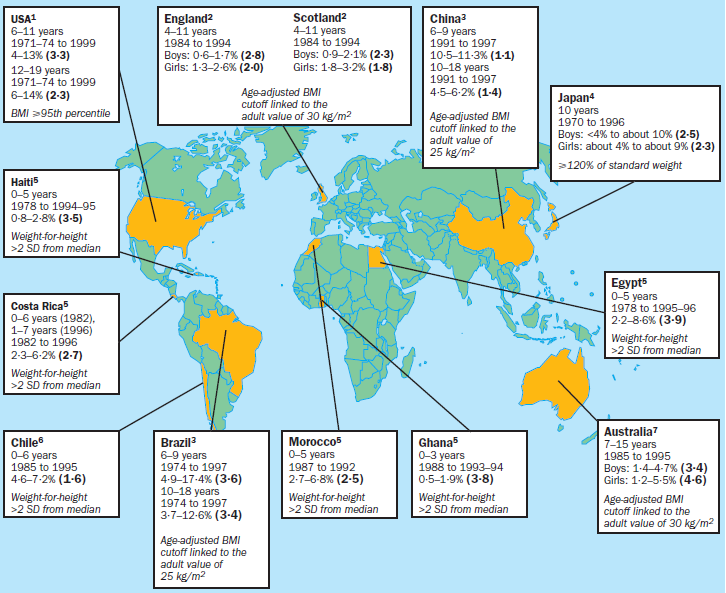
\includegraphics[width=13cm, height=10cm]{immagini/obesity.png}
\caption{Childhood obesity diagram}\label{fig:obesity}
\end{figure}
Historically, a fat child was seen as healthy because he was likely to survive better to illnesses and infections; however, excessive fatness has become one of the most diffused health problem in children. The three experts have underlined how the problem is most common in developed and industrialized nations in which diet has changed radically favouring foods containing saturated and trans fat and with high glycaemic index, typical of fast-food in which also bigger portions are served. Moreover, these foods are also poor of fibre, micronutrients and antioxidants that the body needs for a correct functioning of metabolism. The excessive consuming of these foods brings the child to have health problems such as heart diseases, vascular disorders, hypertension, chronic infiammations and diabete of type 2, illness that in the past was not present in teenagers, but that now has had a rapid spread.\linebreak 

Another important problem that affects the food safety of children is represented by allergies.
According to the data collected by AM Branum and SL Lukacs \cite{FoodallergyUSchildren} it is possible to observe an increasing in cases of all kinds of food allergies including milk, eggs, peanuts, tree nuts, fish, shellfish, soy and wheat of around the 18 per cent on individuals under the age of 18 from the 1997 onwards in US (but we have reasons to believe that this can also be found in all the industrialized world). Reactions to these foods may vary from small diseases to anaphylactic shock that, in severe cases, could lead to death.
The researches have also underlined how, in the same period analized previously, there was also an increasing of hospital discharges (clearly after an hospitalisation) due to allergic reactions as we can see from this barplot.
\begin{figure}[H]
\centering
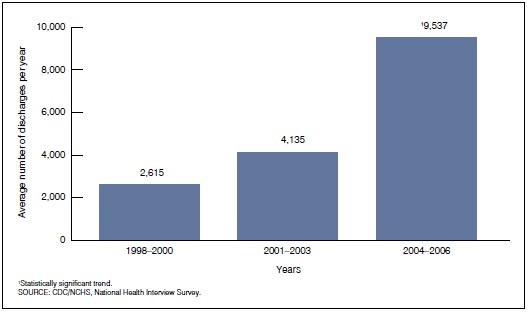
\includegraphics[width=10cm, height=7cm]{immagini/allergybarplot.png}
\caption{Allergy hospital discharges barplot}\label{fig:allergybarplot}
\end{figure}
All these problems that have been reinforced in recent years, lead us to think that it is necessary to support nutrition education and to make it a fundamental thing during childhood and adolescence, in order to empower everyone to a correct care of their health.

\section{Virtual Reality}
"Virtual Reality is electronic simulations of environments experienced via head mounted eye goggles and wired clothing enabling the end user to interact in realistic three-dimensional situations." (Coates, 1992)\\
We can define it using two variables: vividness, richness of an environments representation, and interactivity, extend to which a user can modify form and content of a mediated environment. The vividness is composed by sensory breadth, which refers to the number of sensory dimensions simultaneously presented,and sensory depth, which refers to the resolution within each of these perceptual channels; the interactivity instead is formed by speed, which refers to the rate at which input can be assimilated into the mediated environment, range, which refers to the number of possibilities for action at any given time and mapping, which refers to the ability of a system to map its controls to changes in the mediated environment in a natural and predictable manner.\cite{StefanSeipel} All of them, combined together, influence the telepresence that refers to a set of technologies which allow a user to feel as if he was present at a place different from his true location. So a "virtual reality" is defined as a real or simulated environment in which a perceiver experiences telepresence.\cite{JonathanSteuer}\\
\begin{figure}[H]
\centering
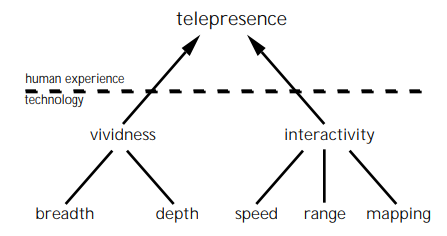
\includegraphics[width=8cm, height=5cm]{immagini/telepresence.png}
\caption{Telepresence infuencing variables}\label{fig:telepresence}
\end{figure}
We focus our project on Wearable Immersive Virtual Reality (WIVR). Immersive is the term that refers to the degree to which a virtual environment submerges the perceptual system of the user in computer-generated stimuli. The more the system captivates the sense and blocks out stimuli from the physical world the more the system is considered immersive.\cite{BioccaDelaney} Wearable indicates that the virtual environment is displayed in specialized small screen: we use a binocular head mounted displays (HMD) which allows to reach a fully immersive experience as we can see from this taxonomy by Muhanna \cite{Muhanna}.
\begin{figure}[H]
\centering
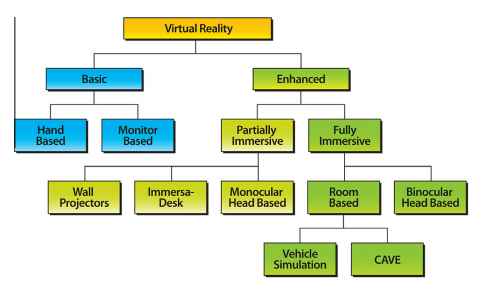
\includegraphics[width=10cm, height=7cm]{immagini/vrtaxonomy.png}
\caption{Virtual Reality taxonomy}\label{fig:vrtaxonomy}
\end{figure}
The HMD "trick" our brain using the principle of stereoscopic vision to simulate the perception of depth and to create 3D images and spaces, the VR has to generate two different images one for each eyes. The lenses of the visor augments the eyes in such a way we can converge the two scenes to obtain only one but that seems to be in the 3 dimensions space. Finally it can track the head movement so when we move it the space updates. 
\begin{figure}[H]
\centering
\begin{minipage}[c]{.40\textwidth}
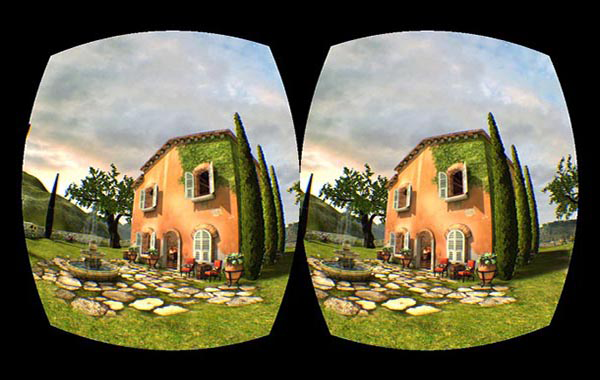
\includegraphics[width=1\textwidth]{immagini/immaginedoppia.png}
\end{minipage}%
\hspace{10mm}%
\begin{minipage}[c]{.40\textwidth}
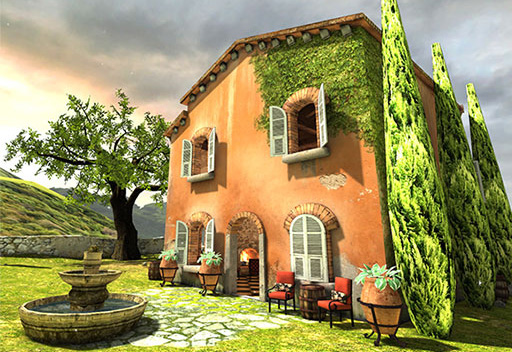
\includegraphics[width=1\textwidth]{immagini/immaginesingola.png}
\end{minipage}
\caption{Stereoscopic image and the correspondent 3D image}\label{fig:vrimages}
\end{figure}
Nowadays HMD are very popular and the costs are in a very big range from a cheap one, like Google Cardboard \cite{Cardboard}, to a more expensive one, like Samsung Gear VR \cite{Gear}, so the VR is for everyone. The VR is also used in a lot of different sectors as we can see in the following graph representing the investments in the 2015 taken from Digi-Capital \cite{DigiCapital}.
\begin{figure}[H]
\centering
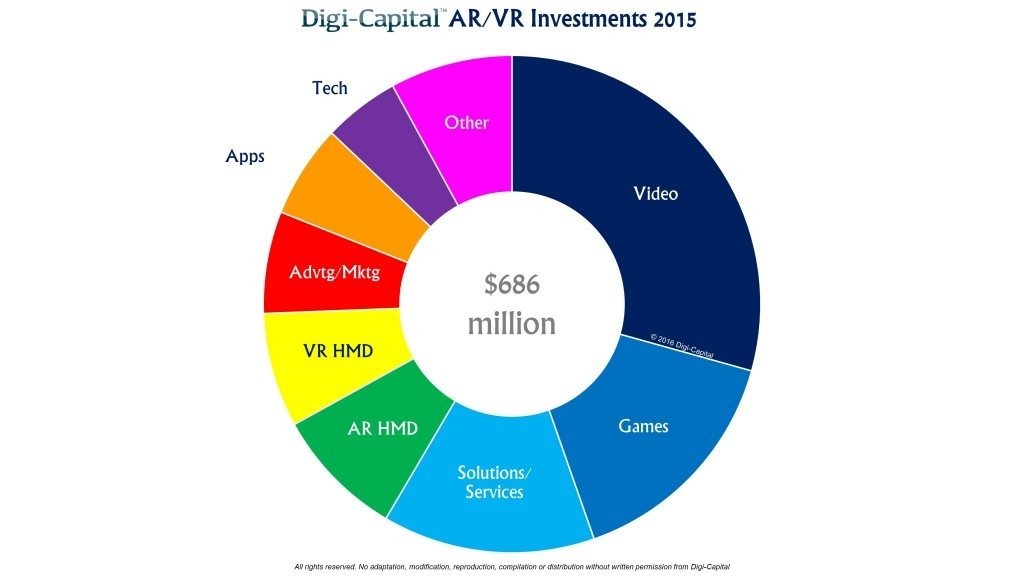
\includegraphics[width=15cm, height=7cm]{immagini/vrsectors.png}
\caption{Virtual Reality investments sectors}\label{fig:investments}
\end{figure}

\section{Touchscreen}
Touchscreen technology is something we have had for a longer time one can think. The first touchscreen device in fact was a radar built in capacitive way and dates back to around 1966. Its invention is due to E. A. Johnson and it works using a sheet of conductive, transparent material with a small current flowing on it. The central computer computes the current at each of the four corners, and when an objects touches the screen, a capacitor is formed between it and the platform and measuring again, the current on the corners the computer is able to approximately compute the point in which there was the touch.\\
At first this technology was abandoned, then in the first 2000s it was used on BlackBerry devices, but the major explosion of touchscreen devices is in the 2007, when Apple releases the first iPhone. \cite{Infante}
From that point on, touchscreen devices become increasingly used (as we can see from the graph below related to phones) and have had an explosive growth due to their main characteristic: the human computer interaction.
\begin{figure}[H]
\centering
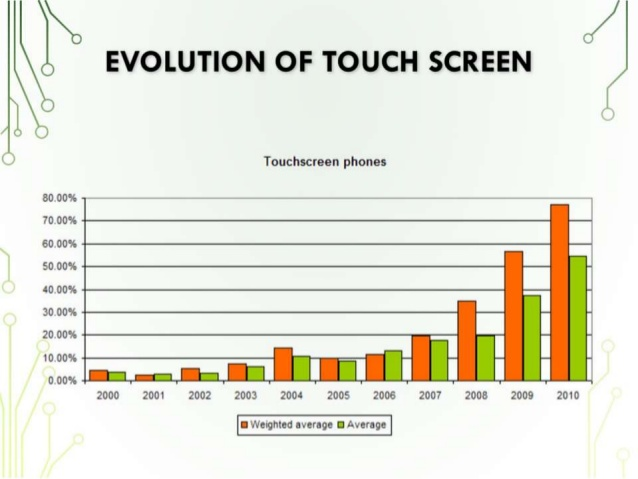
\includegraphics[width=12cm, height=9cm]{immagini/evolutouch.jpg}
\caption{Evolution of touchscreen}\label{fig:evolutouch}
\end{figure}
This interaction could be exploited by the fact that the user could touch directly what he wants without recurring to a third element (like a mouse) and this is particularly appealing because it makes the interaction more intuitive and allows a better usability of the system that is one of the main reasons of the success of this kind of devices. Moreover this improved usability will result in a easier training of people that learns faster and better with reduced costs due to the fact that this technology has grown a lot in recent years and it is no longer excessively expensive and resource-hungry \cite{Creed}.

\section{Neurodevelopmental Disorder}
The term neurodevelopmental disorder, NDD, contains within it all the conditions that are caused by a dysfunction of a part of the brain or nervous system that show some symptoms in the physical and psychological development of the child \cite{EPA}. Among the most common diseases we find Autism, ASD, attention deficit and hyperactivity, ADHD, and Down syndrome \cite{APA}. Children who suffer from these syndromes need help in developing cognitive abilities such as attention and language, social skills such as the ability to relate to others and personal and domestic autonomy skills. Dr. Dorothy Strickland, Department of Computer Science of North Carolina State University, in her treatise on the study of a VR application for autistic children \cite{Dorothy}, states that among the great benefits that can be found are: control on input stimuli, small changes to reach a generalization, safe learning situations, personalized treatment and learning with minimal human interference. In recent years there has been an increase in interest in the use of VR especially in the field of NDDs, \cite{Yufang} and \cite{Garzotto}, as, as stated in \cite{Strickland}, both the strength and limitations of Virtual Reality seem to adapt good for the needs that the learning tools for this type of disability require.\\
\\
As for the spread of these diseases take for example the autism on which there are no certain data, but there is agreement on the fact that the phenomenon is growing. According to the World Health Organization (WHO), ASD affects one child in 160 and recent estimates by the Cdc (Center for Disease Control) indicate that 3 million people are affected by this disorder in the US and about 60 million in world. According to estimates gathered by World Atlas, it would be Japan and Great Britain where autistic disorders occur more often.
\begin{figure}[H]
\centering
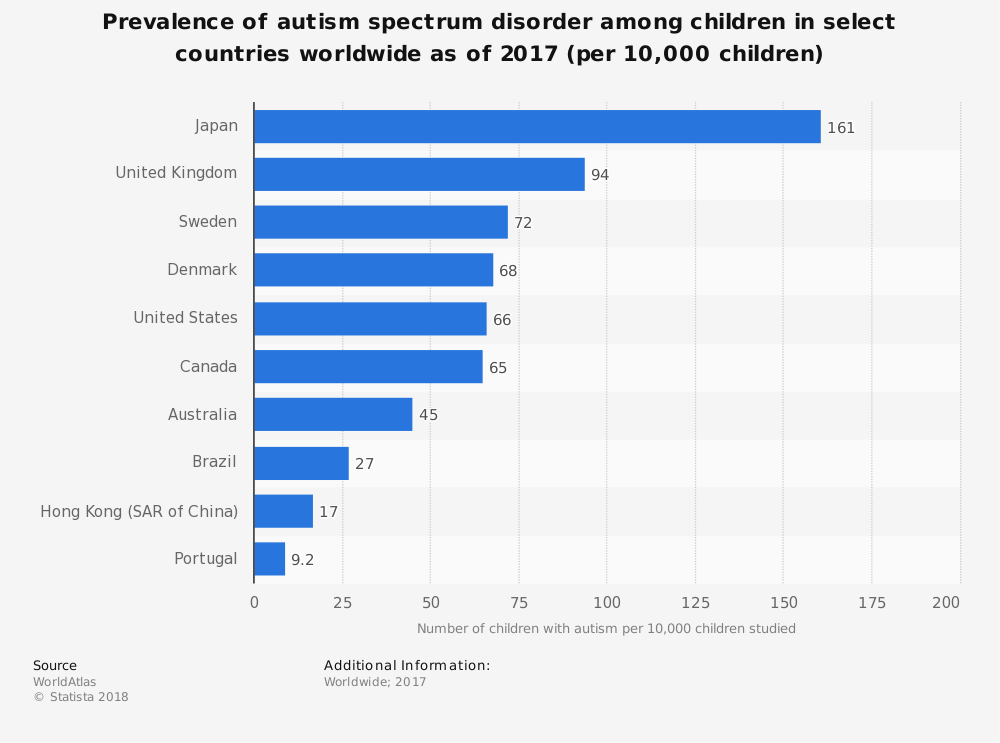
\includegraphics[width=15cm, height=10cm]{immagini/autismo.png}
\caption{Autism diffusion by World Atlas}\label{fig:autism}
\end{figure}

\section{Participatory Design and Therapy}
Over the past six decades, designer have been moving increasingly closer to the future users of what they design. In particular, design is becoming something that is more and more related to what the user needs, this imply the necessity of the collaboration between the experts in field (designers) and the final users (that are usually not experts) leading to what is now called co-design process.\\
The historic user-centred approach, in which designers thought as the user as final objective of their studies, but considered him as a passive entity, have been gradually substituted by the co-design process since the 1970s because people have been giving more importance to activities in which their opinion is required.
\begin{figure}[H]
\centering
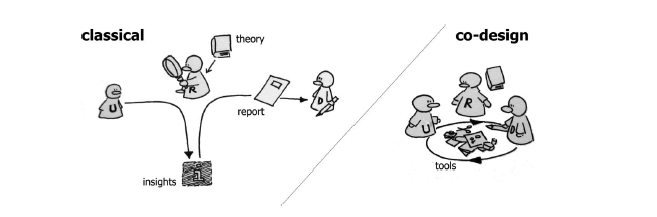
\includegraphics[width=16cm, height=5cm]{immagini/codesign.png}
\caption{Classical approach vs codesign approach}\label{fig:codesign}
\end{figure}
In the classical approach in fact, as we can see in the image above, there were different entities that collaborates to the final design of the product, but the user was considered a passive object of study: researches brings knowledge from theory and developed some more through the observation and interviews. Designer then apply this knowledge to conceptualize the final product. 
In co-creation approach, on the other hand, the roles get mixed-up: the user is involved as "expert of his/her experience" and plays a large role in the knowledge development idea generation and concept development \cite{Elizabeth}.\\
In the field of NDD, this could lead to multiple benefits: in particular, the target user perspective is taken into account since the early design phase and this allow to create something ad-hoc for this kind of people (for example the usage of simple words in explanations, the usage of certain kind of graphic stuffs and so on) and for the participants point of view, this could lead to a greater self-awareness and a more positive social behaviour.



\section{GEA and its Codesign process}
Considering the kind of target our application would have had and the importance of the subject we wanted to treat, we have decided to go through a co-design process which have involved both the final users and the therapists.\\
The starting point of our research were the kind of activities done in food education laboratory: in the first meeting we have observed how these activities are performed and then we have discussed with patients about these activities to hear their opinion and their engagement on them.\\
Then we have proposed our idea to create a virtual reality game based on the learning process provided by those activities that would have been used as a test to verify how much the patients have understood and assimilated the concepts.\\
These concepts have an important role in everyday life because they are related to self-awareness and autonomy in preparing and eating foods that some patients did not have initially and they have to improve their skills on them.\\
The patients have collaborated actively and with a lot of enthusiasm so we have decided to create a first abstract prototype of the application (with mockups and conceptual functioning).\\
In the second meeting we have first exposed our ideas about the three initial mini-games GEA was composed of to the therapist that evaluated their coherence with the food laboratory and their adequacy to the target end user it was thought for. \\
We understood the kind of difficulty required for the game also regarding the kind of interaction the game might have had, so we have changed small stuffs in our first idea, for example we have been informed that not all the users could read and that the presence of a lot of explanation was not useful for the game purpose, so we have thought how to improve the final usefulness of the game.\\
We have then implemented the first prototype of the game, that was tested from twb (ECCETERA, PER ORA IN SOSPESO)
\begin{figure}[H]
\centering
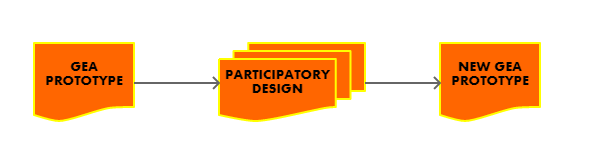
\includegraphics[width=12cm, height=4cm]{immagini/PD.png}
\caption{Phases of the work}\label{fig:phases}
\end{figure}

\section{GEA}
\subsection{Thesi Structure}
The thesis is organized as follows:
\begin{description}
\item[Chapter 1 (State of the art)] In this section we show all the technologies for Virtual Reality, explaining how they works and their relation with NDD people. We present also an instrument very useful for terapist that allow to replicate the smartphone's screen, Google Chromecast, and the touchscreen evolution. Finally we describe the projects already developed about food education.
\item[Chapter 2 (GEA: first prototype)] Here we describe how we elicitate the requirements, which are ours target groups, context, needs, constraints, goals. After that we show the UX design with description of all the app's pages and respective screenshot and flow diagram. Finally we briefly describe the implementation overview.
\item[Chapter 3 (First evaluation)]  
\item[Chapter 4 (GEA: second prototype)]
\item[Chapter 5 (Second evaluation)] 
\item[Chapter 6 (Value proposition)]
\item[Chapter 7 (Challenges)]  
\item[Chapter 8 (Implementation)] We present all the tools used to build up our application and the hardaware and software architecture description.
\item[Chapter 9 (Conclusion)]
\end{description}
At the end of the thesis, two appendices illustrate the materials used during the process
and shows some pictures of the process.
 
\subsection{Origin of the name and mascotte}
We decide to give the name GEA to our application because of two reasons. The first one is that Gea, in the greek mythology, was the personification of the Earth, the mother of all life so she is also the symbol of the nature that recalls the nutrition's topic. The second motivation is that in Italian Gea is the acronym of "Gioco Educazione Alimentare", which translated is "Food Education Game", in this way in the title there is the objective's explanation.\\
We have also designed a mascotte depicting a fairy of fruit and vegetables to leak the message that even the characters recognized by the community as positive eat healthy food; it is in fact dressed with elements such as strawberries like pigtails, pumpkin like a skirt, salad like top and cherries like little bows of shoes.
\begin{figure}[H]
\centering
\begin{minipage}[c]{.40\textwidth}

\includegraphics[width=1\textwidth]{immagini/geamasc.png}
\end{minipage}%
\hspace{10mm}%
\begin{minipage}[c]{.40\textwidth}

\includegraphics[width=1\textwidth]{immagini/GEA.png}
\end{minipage}
\caption{GEA logo and mascotte}\label{fig:logo}
\end{figure}

\chapter{State of the art\label{chap:state-art}}
In our era technology has a foundamental role in almost every field. From the simple communications activities to those related to medical researches, technology is something we cannot do without. It is also a great opportunity in educational field, where it is demonstrated that the so called "stealth learning" (i.e. the help of technologies in educational scope) \cite{Sharp} is a solution to create a greater emotional involvement and that has as a consequence the ability to increase learner's learning opportunities. In our specific case, stealth learning is suitable for the treatment of patients affected by NDD to develop their cognitive, emotional and intellectual skills.

\section{Modern technologies for NDD people}
All the new existing technologies are now helping therapists and families to deal with neurological disabilities. In fact, in addition to virtual reality, smart objects, multisensor environments or smart spaces and conversational agents are used.\\
Smart objects are devices that can interact not only with the user but also with other similar devices and with the surrounding environment. Physical world can be described in terms of three properties \cite{Smart}: awareness (is a smart object to be able to understand events and human activities occurring in the physical world), representation (refers to a smart object's application and programming model) and interaction (denotes the object's ability to converse with the user in terms of input, output, control, and feedback).\\
Examples are Dolphin Sam \cite{Dolphin} and  Huggable \cite{Huggable}. \\
Smart spaces or multisensor environments are rooms in which children can play or interact in a controlled way because they are equipped with techonological items like cameras, smart objects, leds and projectors.
\\
Examples are Magic K room e M4All \cite{M4all}. \\
Conversational agents are devices that can communicate with the user in a manner consistent with what is required: an interaction of the user is answered by the agent who must be with sense.\\
\begin{figure}[H]
\centering
\begin{minipage}[c]{.40\textwidth}
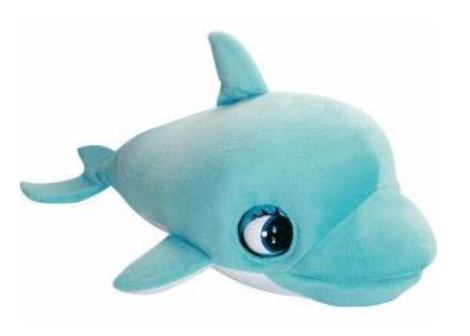
\includegraphics[width=1\textwidth]{immagini/delfino.png}
\end{minipage}%
\hspace{10mm}%
\begin{minipage}[c]{.40\textwidth}
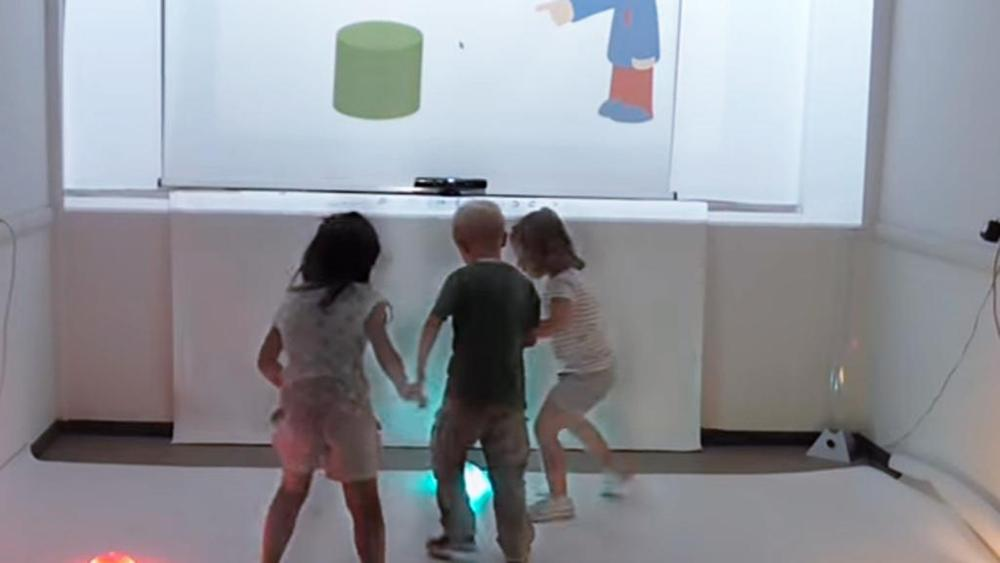
\includegraphics[width=1\textwidth]{immagini/stanzamagica.jpg}
\end{minipage}
\caption{Dolphin Sam and Magic K Room}\label{fig:smartimages}
\end{figure}

\section{Virtual Reality}
The great benefits of using Virtual Reality in an educational and rehabilitation context are now recognized worldwide and tested through various comparative tests between rehabilitation with the use of new technologies and rehabilitation with the use of classical methods \cite{Parsons}, \cite{Reid}, \cite{Wii}. In \cite{Pelagia} a review is carried out on recent literature to support and demonstrate the effectiveness of the use of VR with autistic children and in \cite{Tandra} the effects of a virtual reality game are analyzed to demonstrate the increase in social and emotional activities on a sample of 30 children between 7 and 16 years who suffer from ASD.\\
As previously mentioned, for the development of GEA, an approach that uses Werable Immersive Virtual Reality (WIVR) has been preferred since the possibility of a complete immersion in the environment and the removal of many distractions are the basis of an effective therapy. The user is in a world similar to the real one but safer as there is nothing that can hinder his learning and is reduced to the maximum the "fear" of making mistakes: it is as if the person could "train" the daily life so you can be ready and not catapulted into a world difficult for him. The use of the viewer also allows you to maintain a greater level of concentration because the player can not distract looking elsewhere or perceive the looks and reactions of those around, the only source of disturbance will then be sound. Once this type of games was not accessible to everyone because of the costs of technology and the problems that have been encountered in using it, such as a sense of nausea as sutied by the United States Army in \cite{Eugenia}, but nowadays many steps have been taken and viewers, as well as virtual reality itself, are within everyone's reach.\\
Regarding the technology of Virtual Reality viewers, HMDs, now on the market there is a clear division between two currents: embedded viewers, such as HTC Vive Pro, \cite{Vive}, and modular viewers, such as Google Cardboard, \cite{Cardboard}, and Samsung Gear VR, \cite{Gear}.\\
\textbf{HTC Vive Pro}
\begin{figure}[H]
\centering
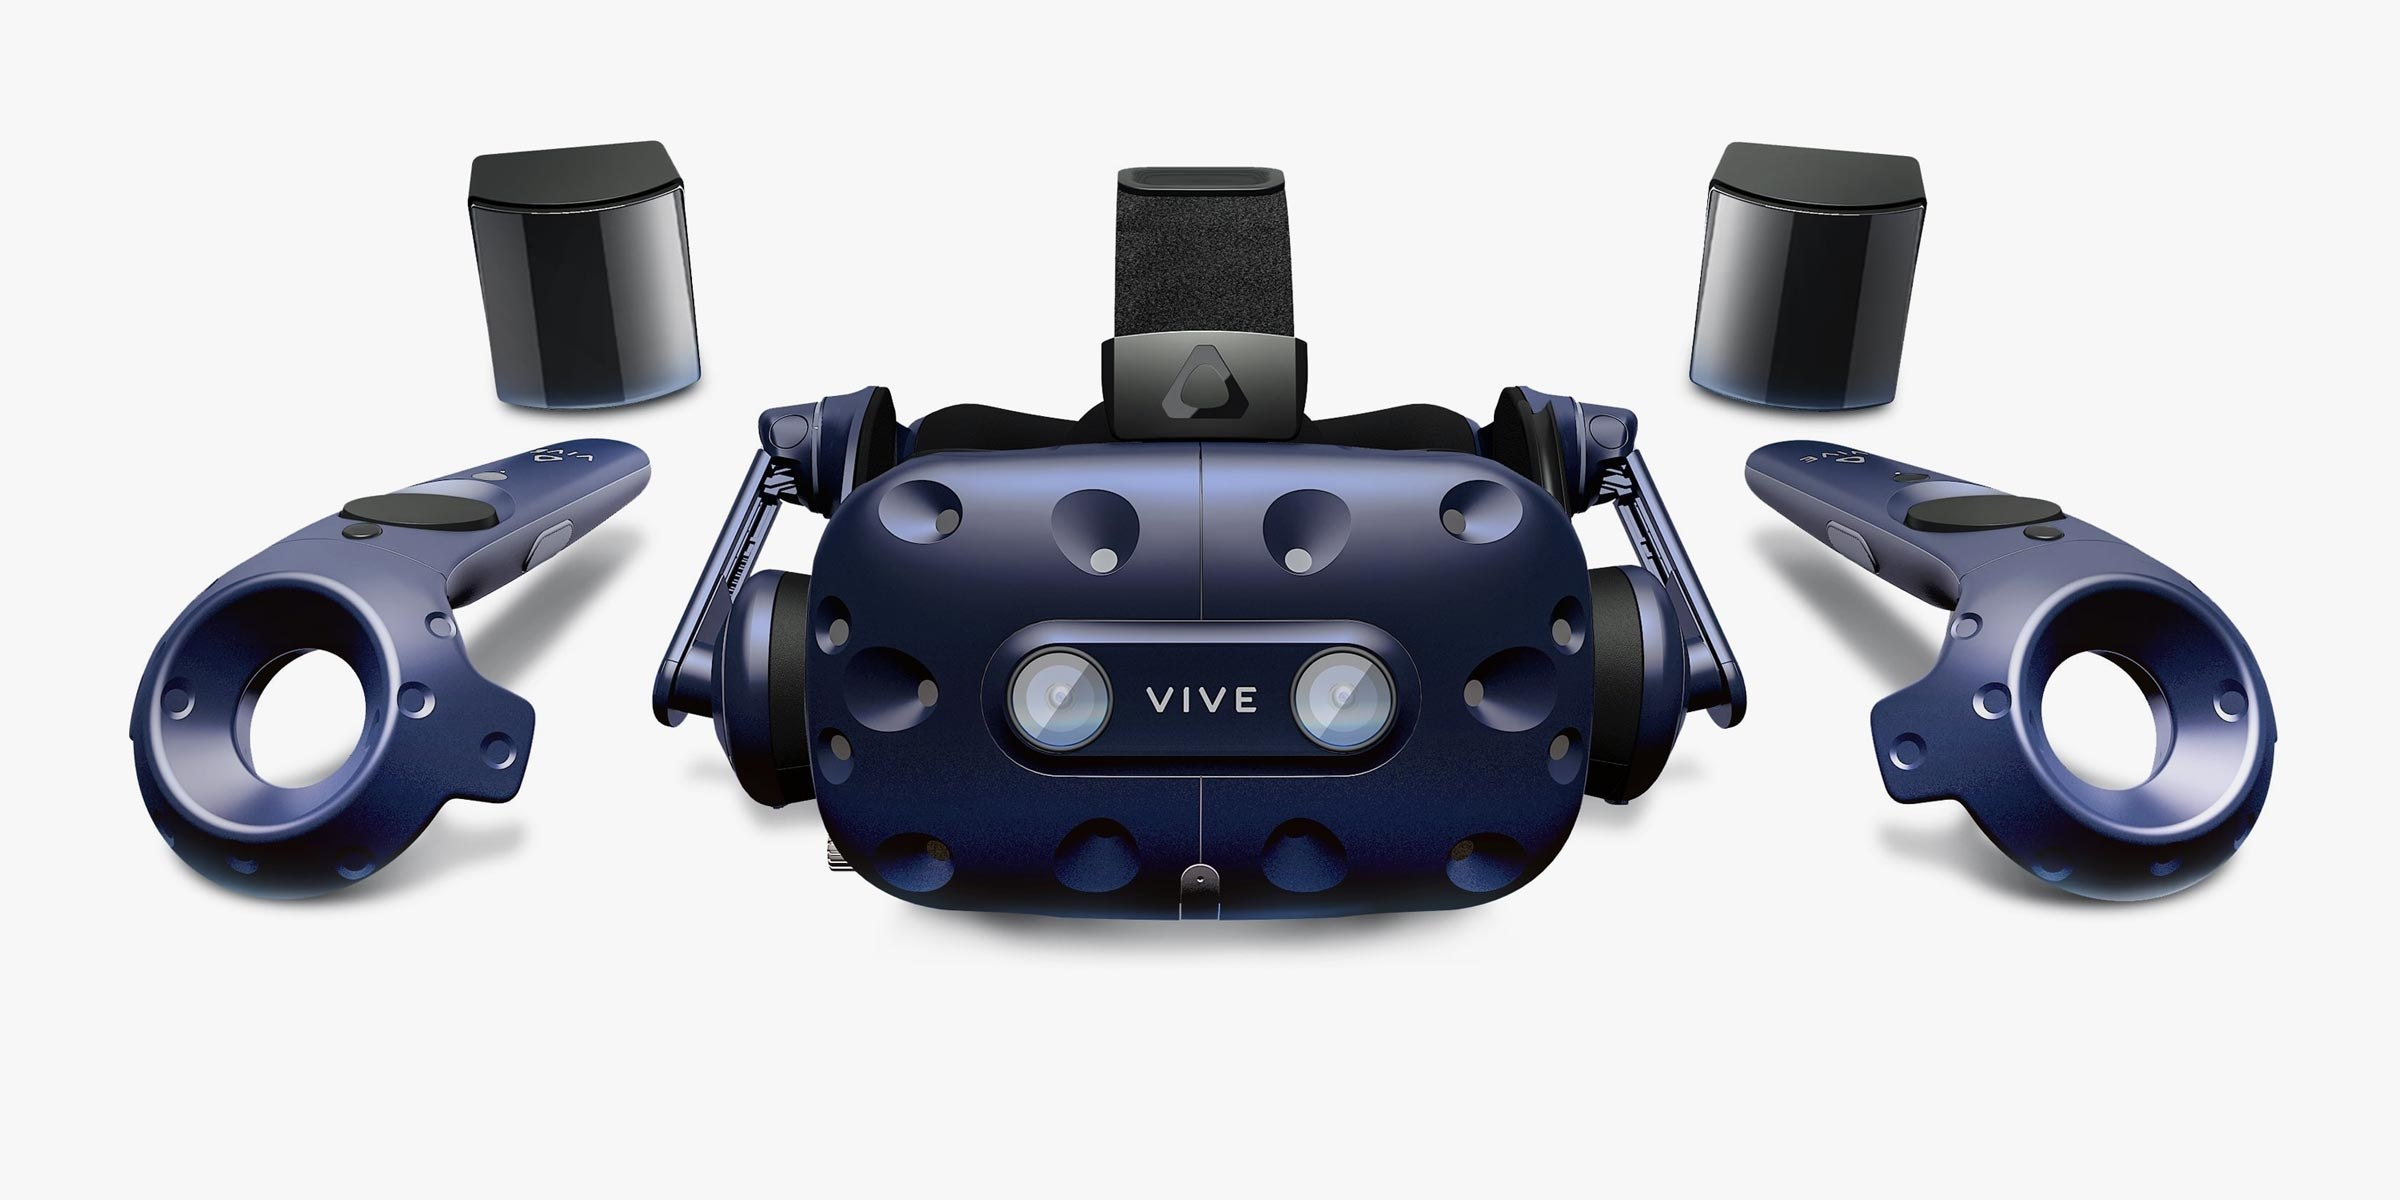
\includegraphics[width=12cm, height=6cm]{immagini/vive.jpg}
\caption{HTC Vive Pro}\label{fig:htcvive}
\end{figure}
HTC Vive Pro is an advanced virtual reality headset developed by HTC and Valve Corporation.The Vive Pro uses two screens, one per eye, each having a display resolution of 1440x1660. The displays are made of AMOLED technology, having a refresh rate of 90 Hz (90 frames per second). The device uses these sensors: SteamVr Tracking, G-Sensor, gyroscope, proximity and IPD sensor. It uses optimized ergonomics and lenses with 110 degrees. But it has a very high cost: 879 euro only the visor and 1399 euro the complete pack (from the official store).\\
\\
\textbf{Google Cardboard}
\begin{figure}[H]
\centering
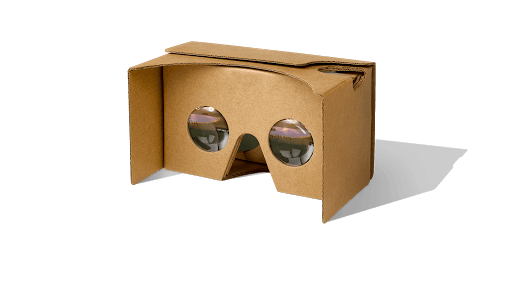
\includegraphics[width=12cm, height=6cm]{immagini/cardboard.png}
\caption{Google Cardboard}\label{fig:cardboard}
\end{figure}
Google Cardboard is composed of two biconvex lenses mounted on a plastic or cardboard frame available in different colors and shapes. The smartphone placed inside this structure shows the visual contents, subdividing them into two-dimensional images with two identical dimensions, and the interaction is obtained through the focused gaze. The user can navigate the virtual world by rotating his head which will consequently rotate the virtual scene projected on the display.\\
\\
\textbf{Samsung Gear VR}
\begin{figure}[H]
\centering
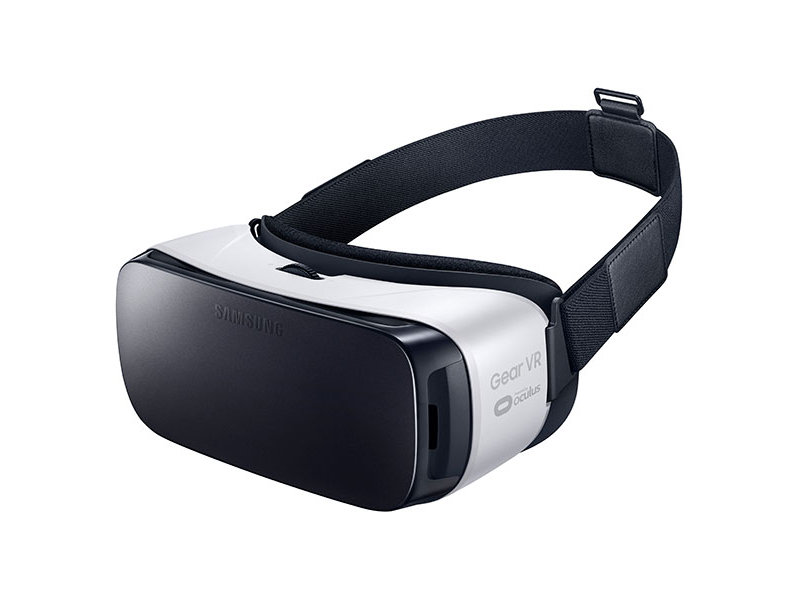
\includegraphics[width=10cm, height=6cm]{immagini/gear.jpg}
\caption{Samsung Gear VR}\label{fig:gearvr}
\end{figure}
Samsung Gear VR is still a modular HMD, produced by Samsung and Oculus VR. It is lightweight and with a good quality of materials,it has accelerometer, gyroscope and proximity Sensor but we can use it only with Samsung smartphones with some specifics. It costs more than Cardboard but it is not so expensive.\\
\\
During the implementation and testing phases of GEA we decided to use the modular visor as it turns out to be the most economical choice on the market and the financial factor is of great importance since the game is designed to be integrated into existing and widely adopted in therapeutic programs.

\section{Touchscreen}
The massive evolution that touchscreen devices have had in recent years, has strongly influenced our way of life. The amount of time a person spend on internet or on electronic devices in general is something that continues to grow every year. From a general point of view this is surely not a good thing because it has a large number of consequences that we have to take care of. \\
This new trend of life surely influences also children, that spend a lot of their time playing games on touchscreen devices, that are more accessible than traditional computers and video games because the motor skills needed to use them are not necessary.\\
\begin{figure}[H]
\centering
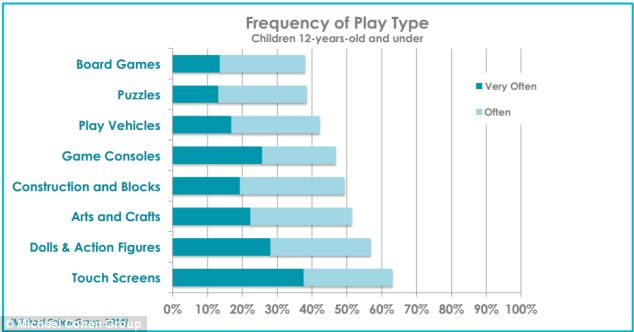
\includegraphics[width=10cm, height=7cm]{immagini/touch.png}
\caption{Time spent by children at playing games}\label{fig:timegames}
\end{figure}
Despite this kind of behaviour is largely criticized and not recommended by doctors and psychologists, the experiment conducted by B. Huber, J. Tarasuik, M.N. Antoniou, C. Garrett, S.J. Bowe and J. Kaufman \cite{Huber} demonstrated that children could learn from touchscreen educational games and apply this knowledge on physical problems. In fact there're a lot of applications thought for this purpose that help children to develop memory, problem-solving and executive functioning skills that could then be applied to real-world problems. The experiment shows substantially that there's no difference in learning for children that use real objects from those who learn only on touchscreen application. In particular, as observed by M.J. Mayo \cite{Mayo}, games could involve children more easily due to the presence of images, animations and sounds. Moreover, they're particularly adept at dosing information delivery. On a touchscreen application it is easy to complicate things and to add visual elements as the difficulty increases, while mantaining the focus on a small area that avoid extraneous distractions, so these educational games seems to be effective in enhancing motivation and increasing children interest in subject matter that leads to more effective learning \cite{Annetta}. 

\section{Google Chromecast}
Google Chromecast, \cite{Chromecast}, is a support device that we need for our application in order to exploit all its functionalities. It is a device that allows to send audio and video streams from a screen to another, without any wire through a technology called Google Cast.
\begin{figure}[H]
\centering
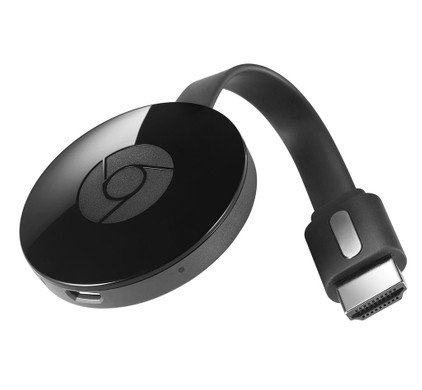
\includegraphics[width=7cm, height=6cm]{immagini/chromecast.jpg}
\caption{Google Chromecast}\label{fig:chromecast}
\end{figure}
In particular the link between the smartphone or tablet (what we want to replicate) and the Chromecast is done through a common wi-fi connection and Google Home app, then from the Chromecast to the television or computer (where we want to see the replication) through the direct connection of the key from the HDMI port. In this way we can replicate live contents and see what's going on inside the VR application or in the touchscreen one. \cite{Jared} \\
This technology, as said before, is essential for the purpose of our application, because we need it in order to allow group training and the possibility for the therapist to give explanation on what to do during the experience, that is one of the main feature of our application. 


\section{Projects about food education}
In the specific field of food education, we could find different kinds of game developed for touchscreen devices. In particular one example is the Food pyramid game developed by the Colorado State University \cite{Serrano} as a game to teach children what are the five main food groups and how to apply this knowledge to plan meal and snacks in order to increase their self-efficacy. This game is composed by various challenges regarding the food pyramid, and the researches has concluded that a game composed with a challenge is more effective that one based on a storyline.\\
Important companies are committed every year to the promotion and development of interactive educational games for children in this field both for the school and for the home, it is an example Nestl\'e with the project "Nutrikid", \cite{Nutrikid}, prepared with advice Scientific Committee of the NFI, Nutrition Foundation of Italy. As they read from their website "The Nutrition Foundation of Italy, was constituted legally as a non-profit association in December 1976, with the aim of activating interactions and collaborations with government bodies, universities and industry to contribute the development of scientific research, the exchange of information in the field of nutrition and the promotion of interdisciplinary research in this field.", \cite{NFI}, for this reason we have drawn great inspiration from it during the development of GEA. Other projects in this field are continually promoted by the FEI, Food Education Italy, a foundation of accredited participation at the Ministry of Education, University Research, which lives on voluntary contributions and is involved in helping schools and teachers to develop their role of food educators, \cite{FEI}.\\
Instead, as regards the specific field of food allergies, the state of the art appears to be scarce. It is possible to find, as applications, on the App Store and Play Store, only two games in this regard and both are in English, they are "Wizdy Diner" and "Allergy Reality" developed with touch screen technology and for PC. \cite{Wizdy} and \cite{Allergy}


\chapter{Target groups, Needs and Requirements\label{chap:target-need-req}}
\section{Requirements elicitation}
\section{Onlus varie}
\section{Main target groups}
There are three main categories of stakeholders involved in our application:
\begin{itemize}
\item The first group is composed by children with NDD because they can have great benefits in using it. It can also be used by children not affected by this syndrome but it can result "simple".
\item In the second group there are therapists, in hospitals or organizations, educators and all the other people that have to teach food education to NDD children. They can integrate their lessons with a game session using GEA to improve understanding and have a feedback on children's knowledge so it can be used in specialized centers or schools but also at home because you need only few technological instruments and not very high capabilities in computer science.
\item The tird group encloses developpers, managers, researchers, designers, VR companies and all the people that can be affected by GEA diffusion and results.
\end{itemize} 
\section{Context and need addressed}
\section{Constraints}
\section{Goals}
\section{Requirements}
elencati

\chapter{Design\label{chap:design}}
\section{General approach}
\section{Descrizione singole parti}
\section{Scenarios}
\section{UX}
\subsection{Site maps}
\subsection{Pages}
\subsection{Use cases}
activity diagram

\chapter{Implementation\label{chap:implementation}}
\section{Tools}
\section{Hardware Architecture}
\section{Software Architecture}

\chapter{Content issues\label{chap:issues}}
Problems and solutions con tabella pro e contro.

\chapter{Evaluation\label{chap:evaluation}}
Fasi varie strutturate con: objectives, participants, test setup, introduction to the test, test procedure, feedback, test results and conclusions.


\chapter{Value proposition\label{chap:value}}
\section{Evaluation method}
\section{Evaluation results}

\chapter{Future work\label{chap:future}}



\bibliographystyle{plain}
\bibliography{bibliography}
\addcontentsline{toc}{chapter}{Bibliography}

\appendix

\chapter{First appendix - User manual\label{app:first-appendix}}



\chapter{Second appendix - Questionar\label{app:second-appendix}}


\cleardoublepage

\end{document}
